% \documentclass[12pt, a4paper, oneside]{ctexart}
\documentclass[12pt, oneside]{ctexart}
\usepackage{amsmath, amsthm, amssymb, appendix, bm, color, enumerate, framed, graphicx, longtable, mathrsfs, subfigure, tikz, ulem}
% \usepackage[dvipsnames]{xcolor}
% \usepackage{geometry}
\usepackage[a4paper, total={145mm,210mm}]{geometry}
\geometry{left=2.54cm,right=2.54cm,top=3.18cm,bottom=3.18cm}
\usepackage{pdfpages}

%按章节编号
\numberwithin{figure}{section}
\numberwithin{table}{section}

% 超链接设置
\usepackage{hyperref}
\hypersetup{  
    colorlinks = true,     % 更改链接颜色  
    linkcolor = purple,    % 链接颜色  
    urlcolor = blue,       % URL 颜色  
    citecolor = darkgreen, % 引用颜色  
    % underline = true,  
    linkbordercolor = red,
}
% \hypersetup{colorlinks=true,linkcolor=black}


%代码包设置
\usepackage{listings}
\lstset{
    basicstyle          =   \sffamily,          % 基本代码风格
    keywordstyle        =   \bfseries,          % 关键字风格
    commentstyle        =   \rmfamily\itshape,  % 注释的风格,斜体
    stringstyle         =   \ttfamily,  % 字符串风格
    flexiblecolumns,                % 别问为什么,加上这个
    numbers             =   left,   % 行号的位置在左边
    showspaces          =   false,  % 是否显示空格,显示了有点乱,所以不现实了
    numberstyle         =   \zihao{-5}\ttfamily,    % 行号的样式,小五号,tt等宽字体
    showstringspaces    =   false,
    captionpos          =   t,      % 这段代码的名字所呈现的位置,t指的是top上面
    frame               =   lrtb,   % 显示边框
}
% \lstdefinestyle{C}{
%     language        =   C, % 语言选C
%     basicstyle      =   \zihao{-5}\ttfamily,
%     numberstyle     =   \zihao{-5}\ttfamily,
%     keywordstyle    =   \color{blue},
%     keywordstyle    =   [2] \color{teal},
%     stringstyle     =   \color{magenta},
%     commentstyle    =   \color{red}\ttfamily,
%     breaklines      =   true,   % 自动换行,建议不要写太长的行
%     columns         =   fixed,  % 如果不加这一句,字间距就不固定,很丑,必须加
%     basewidth       =   0.5em,
% }
\lstdefinestyle{SQL}{
    language        =   SQL, % 语言选C
    basicstyle      =   \zihao{-5}\ttfamily,
    numberstyle     =   \zihao{-5}\ttfamily,
    keywordstyle    =   \color{blue},
    keywordstyle    =   [2] \color{teal},
    stringstyle     =   \color{magenta},
    commentstyle    =   \color{red}\ttfamily,
    breaklines      =   true,   % 自动换行,建议不要写太长的行
    columns         =   fixed,  % 如果不加这一句,字间距就不固定,很丑,必须加
    basewidth       =   0.5em,
}


% 设置思源宋体为中文字体
\setCJKsansfont{Source Han Serif SC}

% 设置思源黑体为中文字体
\setCJKsansfont{Source Han Sans SC}

% 设置arev为英文字体
\setsansfont{Arev Sans}

% 字体颜色
\def\red{\color{red}}
\def\blue{\color{blue}}
\def\black{\color{black}}
\def\green{\color{green}}

\CTEXsetup[format={\Large\bfseries}]{section}

\renewcommand{\abstractname}{\Large\textbf{概览}}

\begin{document}

\thispagestyle{empty}

\begin{figure}[t]
    \centering
    
\includegraphics[width=13cm]{images/logo.png}
\end{figure}

\vspace*{\fill}
    \begin{center}
        \Huge\textbf{数据库原理实践 \\ 教师课程信息管理系统}
    \end{center}
\vspace*{\fill}

\begin{table}[b]
    \centering
    \large
    \begin{tabular}{ll}
    \textbf{课程:} & 数据库原理 \\
    \textbf{班级:} & 1621402 \\
    \textbf{姓名:} & 黄钰轩 \\
    \textbf{学号:} & 162140222 \\
    \textbf{教师:} & 郑吉平 \\
    \textbf{学期:} & 2023-2024 春季 \\
    \end{tabular}
\end{table}

\newpage

\thispagestyle{empty}
\begin{abstract}
    该门课程旨在理解 SQL 定义功能、熟练掌握 SQL 操纵功能、了解 SQL 数据控制功能. 在本项目中,我选用了 \href{https://www.postgresql.org/}{PostgreSQL} 作为数据库,同时使用 Rust 语言中的 \href{https://crates.io/crates/sqlx}{sqlx crate} 访问阿里云数据库 RDS PostgreSQL Serveless, 同时使用 \href{https://www.pgadmin.org/}{pgAdmin 4} 与 \href{https://www.jetbrains.com/clion/}{CLion} 连接数据库,构建了一个小型的教师课程数据管理系统. 该项目是一个 Rust 全栈开发项目,拥有完整的前后端功能,后端使用 \href{https://actix.rs/}{Actix Web} 框架,前端使用模板引擎\href{https://keats.github.io/tera/}{Tera} 与 \href{https://www.rust-lang.org/what/wasm}{Web­Assembly} 构建,数据库使用阿里云数据库 RDS PostgreSQL Serveless. 项目已开源,地址为 \href{https://github.com/Cresc3ntRose/coursedb}{coursedb}. 在开发过程中,我的操作系统配置为 Ubuntu 20.04 LTS 与 macOS Sonoma 14.5, 请尽量避免在 Windows 环境下运行项目代码.
    \par\textbf{关键词:} 数据库原理, SQL, PostgreSQL, Rust, Actix Web, Web­Assembly.
\end{abstract}

\newpage
\pagenumbering{Roman}
\setcounter{page}{1}
\tableofcontents
\newpage
\setcounter{page}{1}
\pagenumbering{arabic}

\section*{世界诞生的前夜: 开发环境配置}
下载 \href{https://www.pgadmin.org/}{pgAdmin 4} 与 \href{https://www.jetbrains.com/clion/}{CLion},并与阿里云数据库 RDS PostgreSQL Serveless连接. 在 RDS 管理控制台创建高权限账号 \texttt{demo\_teacher}.
\begin{figure}[!htbp]
    \centering
    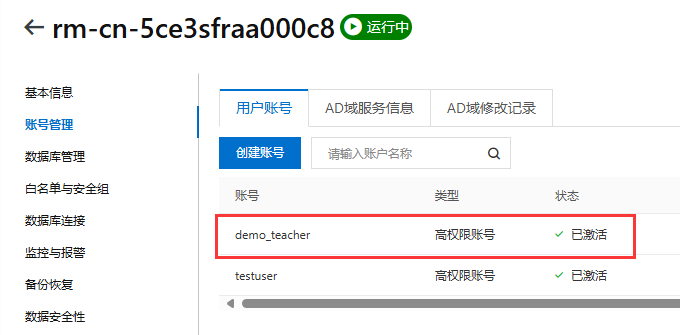
\includegraphics[width=13cm]{images/sec0/创建账号.png}
\end{figure}

接下来创建数据库 \texttt{tutorial} 并与账号 \texttt{demo\_teacher} 绑定.
\begin{figure}[!htbp]
    \centering
    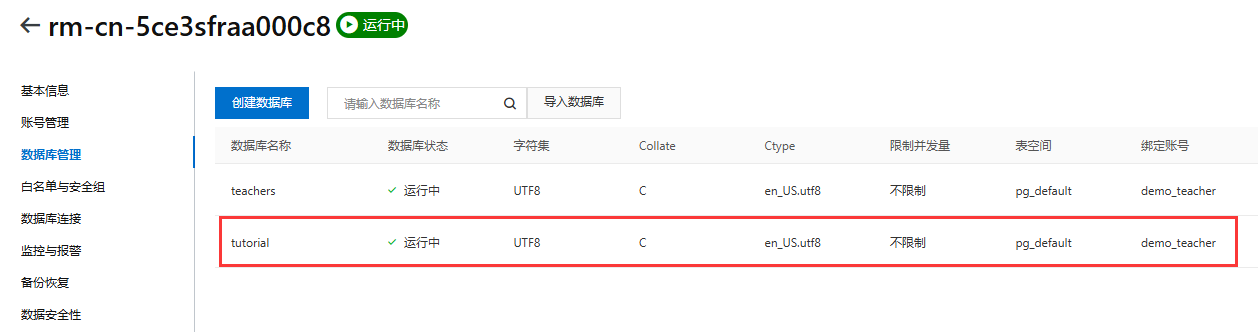
\includegraphics[width=13cm]{images/sec0/创建数据库.png}
\end{figure}

在 pgAdmin 4 与 CLion 中连接数据库,即可完成环境配置.

\newpage

\section{需求分析}

\subsection{应用需求分析}

本项目旨在设计和实现一个课程数据库系统,以满足教育机构对课程管理的需求. 该系统应能够提供以下功能:
\begin{itemize}
    \item 课程信息管理: 能够添加、修改和删除课程信息,包括课程名称、课程代码、教师代码、开课时间等.
    \item 教师信息管理: 能够添加、修改和删除教师信息,包括教师姓名、照片链接、个人简介等.
\end{itemize}

\subsection{数据字典}

\textbf{课程表(Courses)}
\begin{itemize}
    \item \textbf{teacher\_id}:教师ID(整型,外键,指向教师表的ID)
    \item \textbf{id}:课程ID(整型,主键)
    \item \textbf{name}:课程名称(字符串)
    \item \textbf{time}:开课时间(日期时间,可选)
    \item \textbf{description}:课程描述(字符串,可选)
    \item \textbf{format}:授课格式(字符串,可选)
    \item \textbf{structure}:课程结构(字符串,可选)
    \item \textbf{duration}:课程持续时间(字符串,可选)
    \item \textbf{price}:课程价格(整型,可选)
    \item \textbf{language}:授课语言(字符串,可选)
    \item \textbf{level}:课程难度级别(字符串,可选)
\end{itemize}

\textbf{教师表(Teachers)}
\begin{itemize}
    \item \textbf{id}:教师ID(整型,主键)
    \item \textbf{name}:教师姓名(字符串)
    \item \textbf{picture\_url}:教师照片链接(字符串)
    \item \textbf{profile}:教师个人简介(字符串)
\end{itemize}

\subsection{数据结构}

基于上述数据字典,我们可以设计以下数据结构:
\begin{itemize}
    \item \textbf{课程表(Courses)}:存储课程的详细信息,包括课程ID、教师ID、课程名称、开课时间等.
    \item \textbf{教师表(Teachers)}:存储教师的详细信息,包括教师ID、姓名、照片链接和个人简介.
\end{itemize}

这些表通过\textbf{teacher\_id}字段将课程与教师关联起来,形成一个完整的课程数据库系统.

\section{概念结构设计}

\subsection{$E-R$模型实体及关系}

该系统涉及以下几个实体:
\begin{enumerate}[(1)]
    \item \textbf{课程实体(Courses)}:包括课程编号id、授课教师teacher\_id、课程名称name、开课时间time等属性.
    \item \textbf{教师实体(Teachers)}:包括教师编号id、姓名name、照片链接picture\_url、个人简介profile四个属性属性.
\end{enumerate}
这些实体之间的关系为:
\begin{enumerate}[(1)]
    \item 一门课程只能由一个教师讲授.
    \item 一个教师可以讲授多门课程.
\end{enumerate}

\subsection{设计$E-R$图}

$E-R$图如下所示:
\begin{figure}[!htbp]
    \centering
    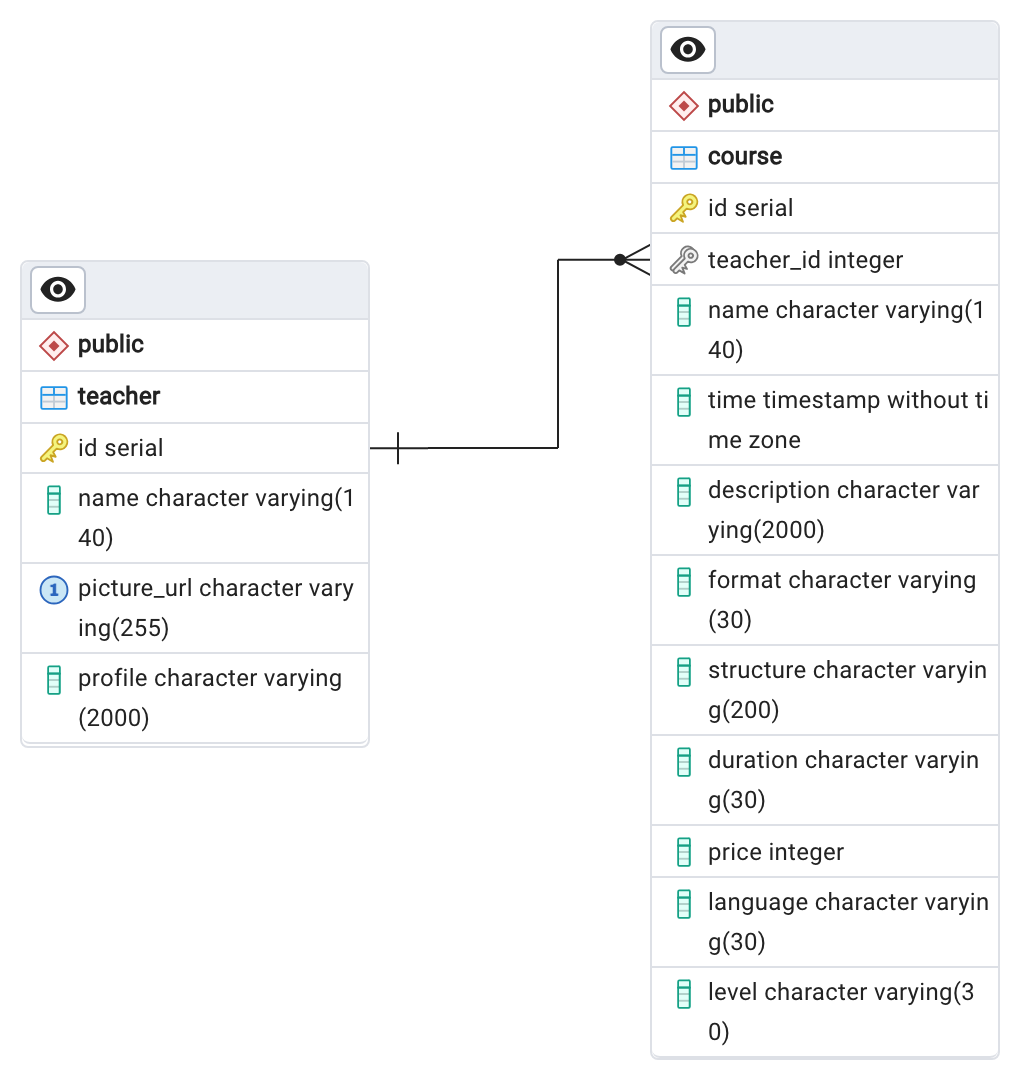
\includegraphics[height = 10cm]{images/sec2/ERD.png}
\end{figure}

\section{逻辑结构设计}

\subsection{$E-R$图转换为关系模型}

根据$E-R$图,我们可以将实体和关系转换为关系模型:
\begin{figure}[htbp]
    \centering
    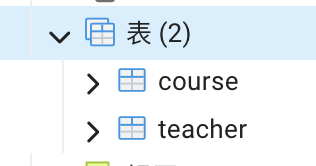
\includegraphics[height = 3cm]{images/sec3/table.png}
\end{figure}

\section{物理结构设计}

\subsection{表的建立}

分别建立teacher与course两个表.
\newpage
首先建立教师表 teacher, 代码详见\hyperref[teacher_query]{附录}.
\begin{figure}[!htbp]
    \centering
    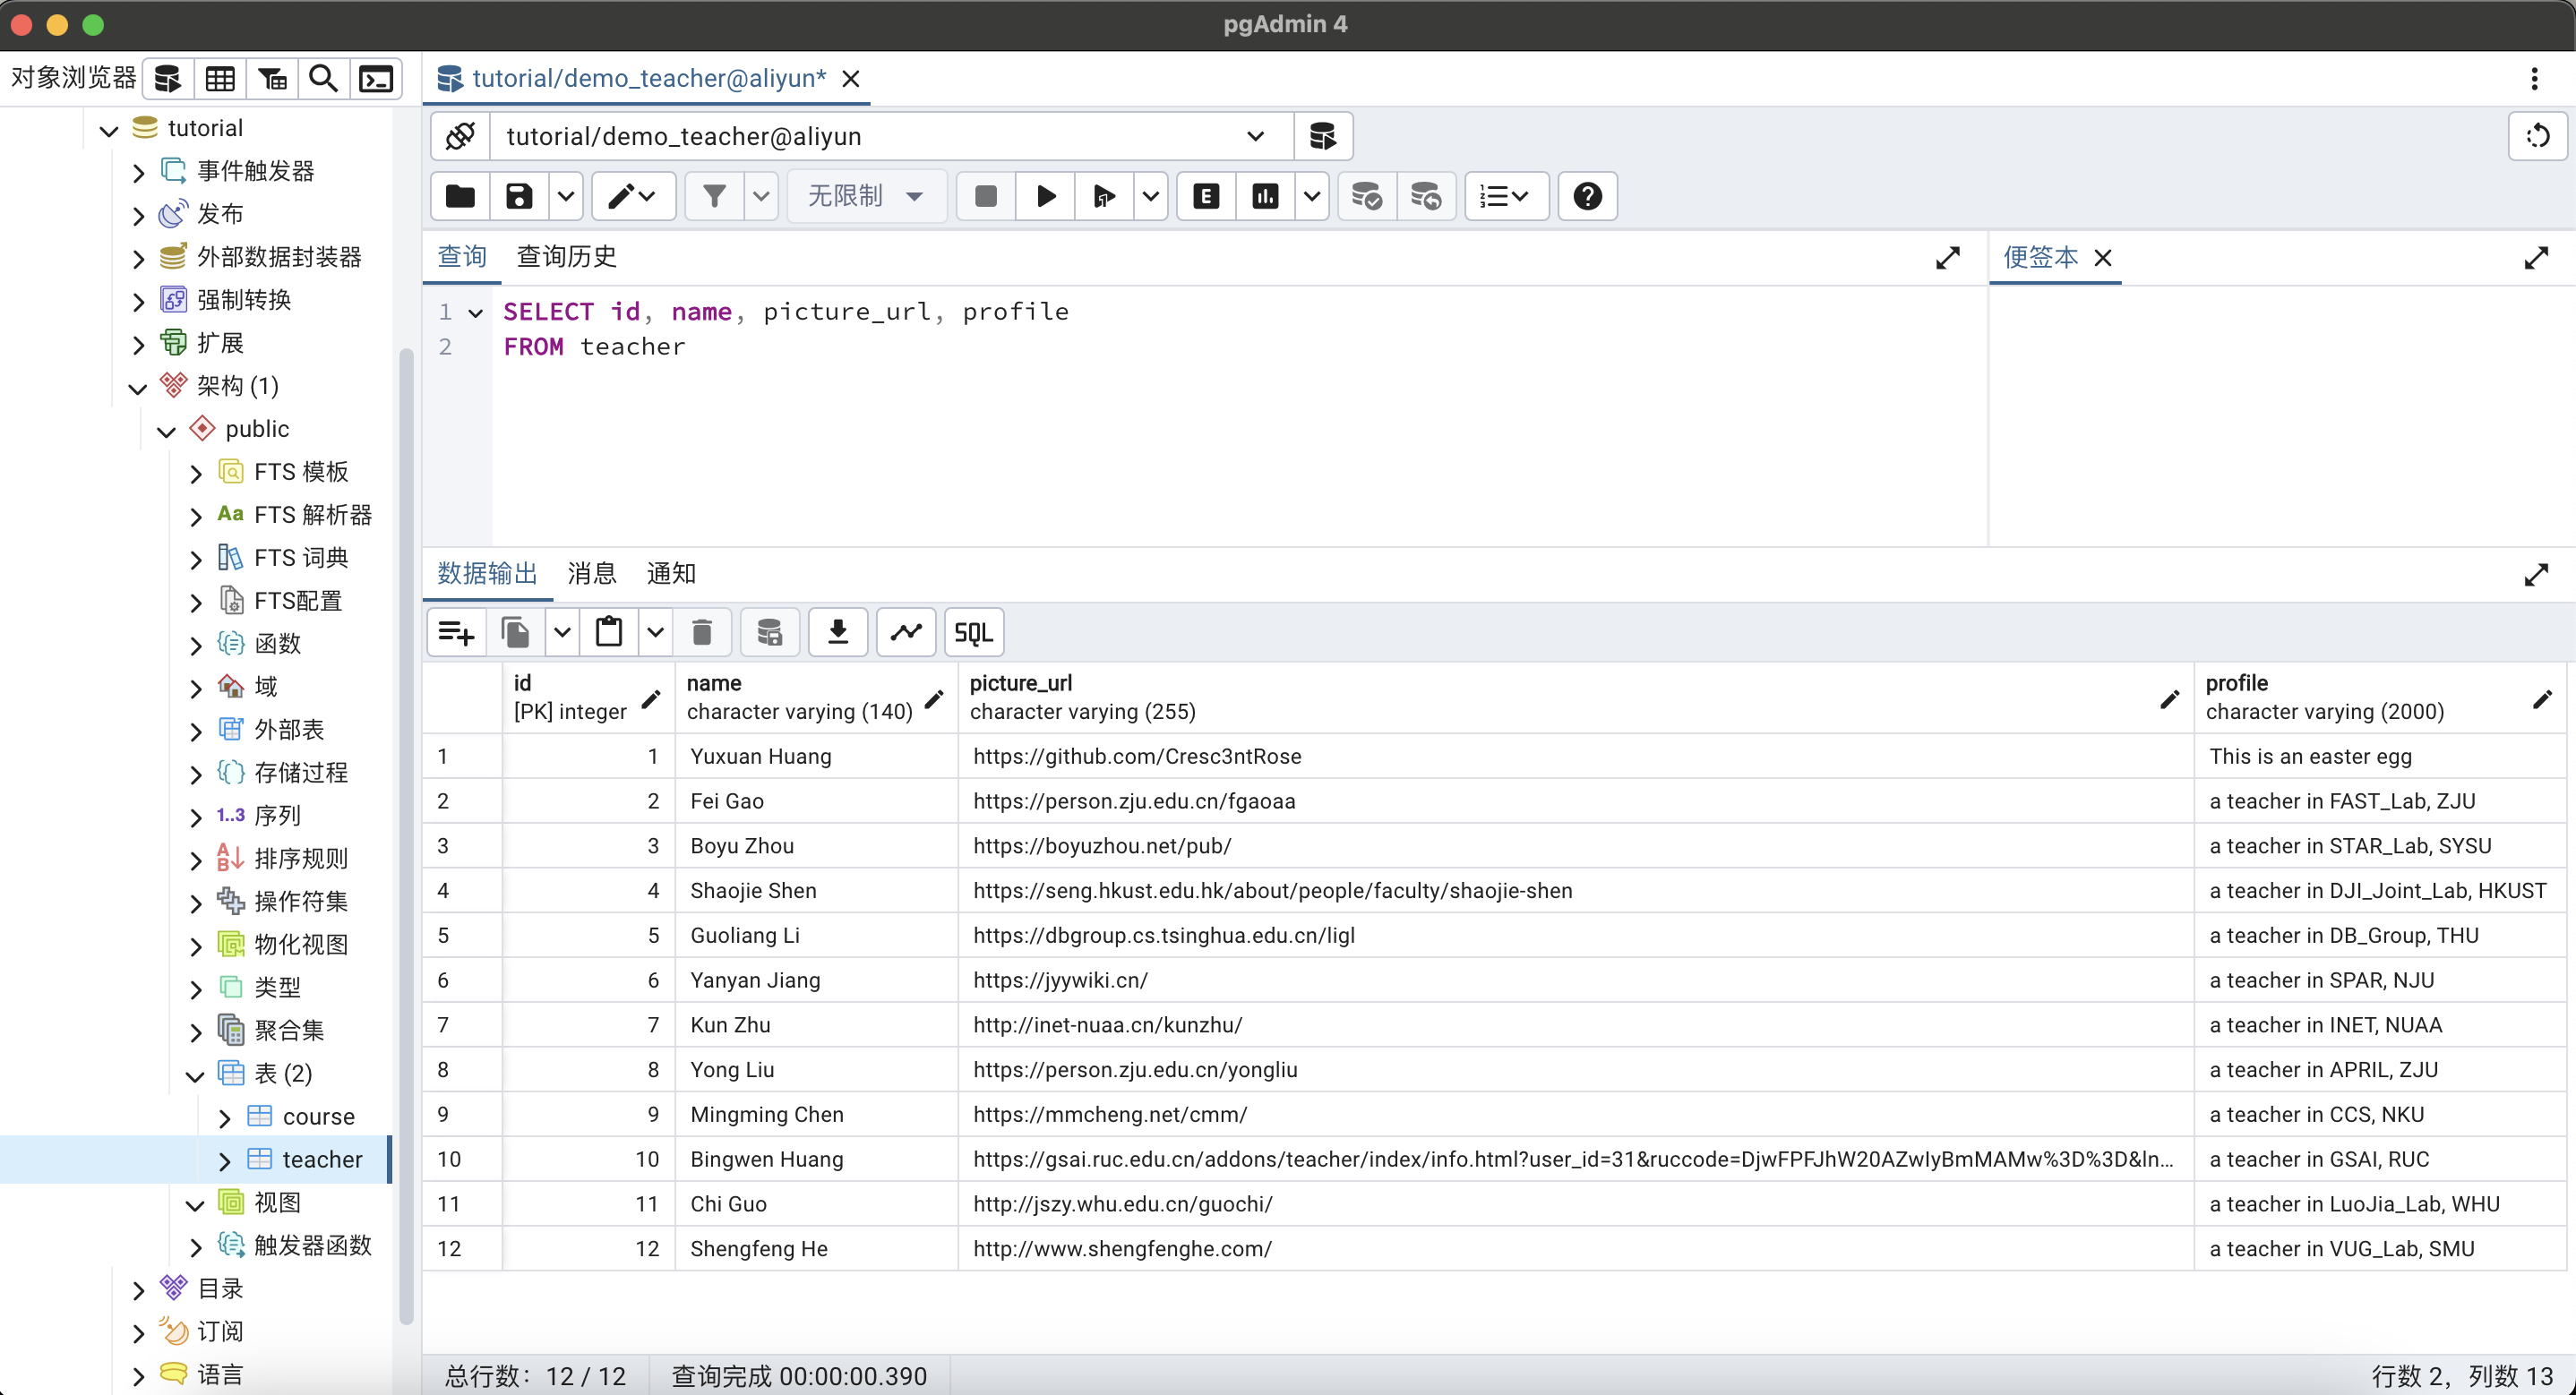
\includegraphics[width=13cm]{images/sec4/teacher.png}
    \caption{teacher表}
\end{figure}

然后建立课程表 course, 代码详见\hyperref[course_query]{附录}.
\begin{figure}[!htbp]
    \centering
    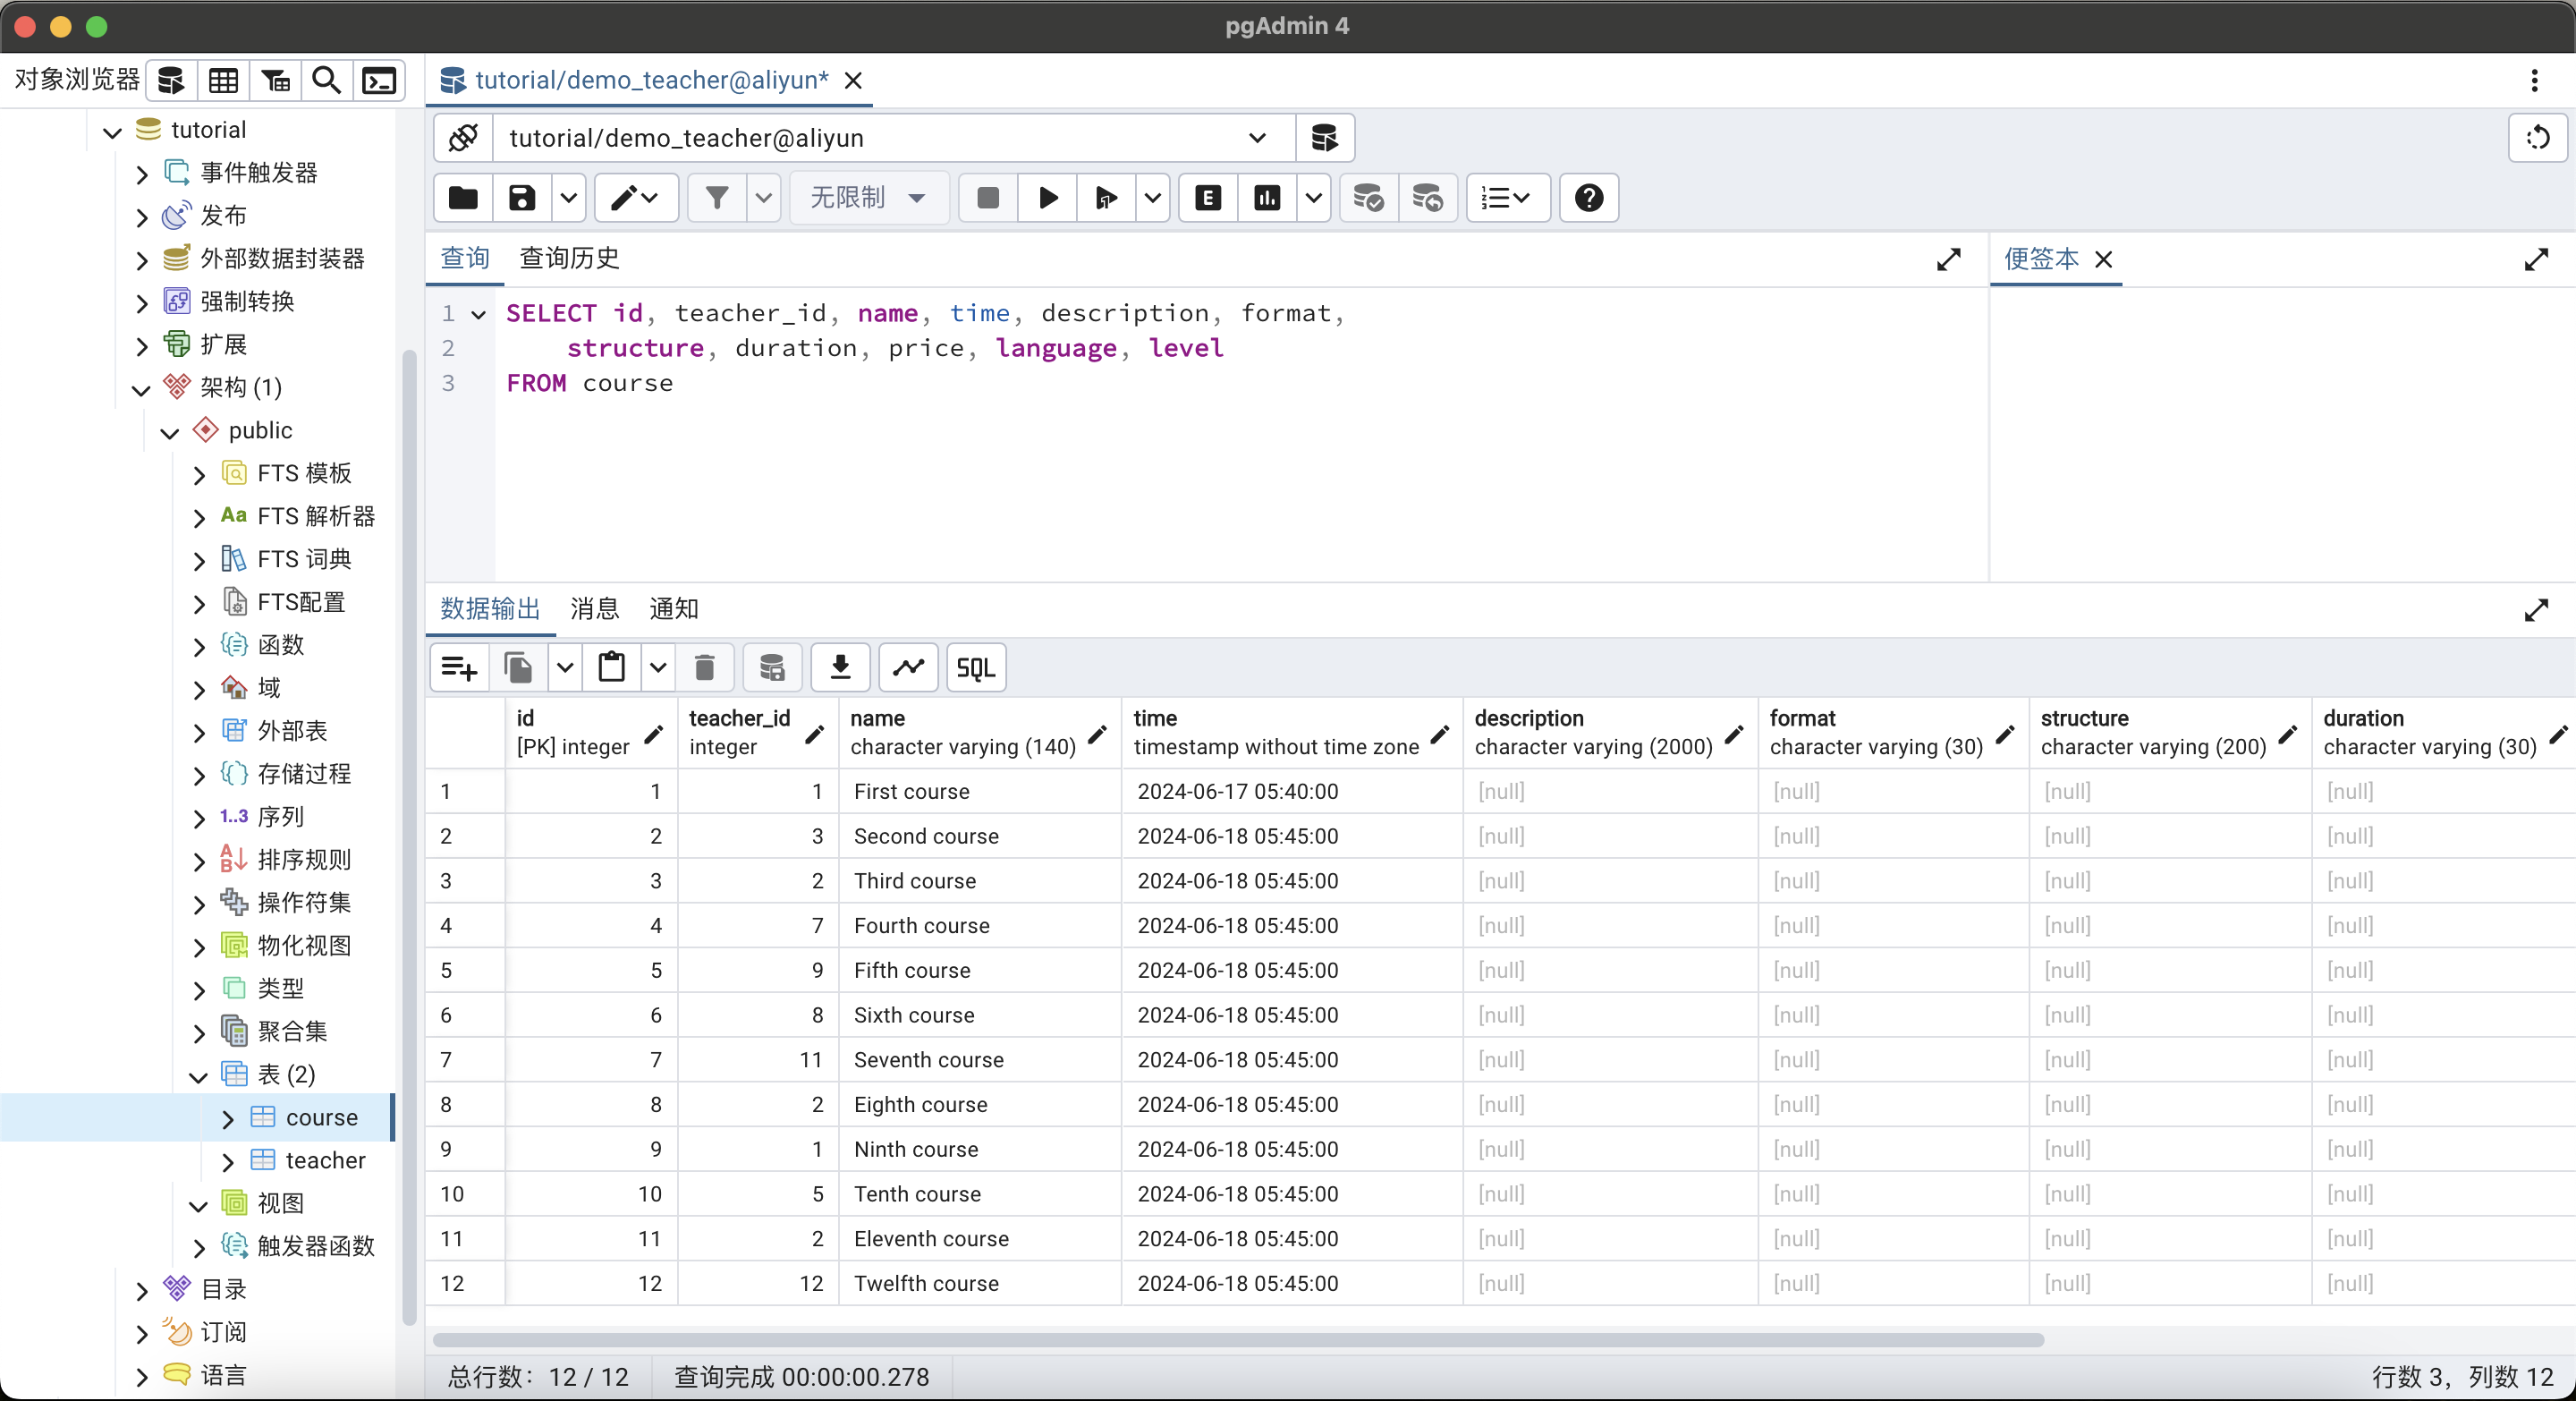
\includegraphics[width=13cm]{images/sec4/course.png}
    \caption{course表}
\end{figure}

\section{数据库实施与维护}

\subsection{数据导入}

通过 pgAdmin 4 中的 SQL 查询功能导入数据到数据库中,以便后续操作,运行结果如下:
\begin{figure}[!htbp]
    \centering
    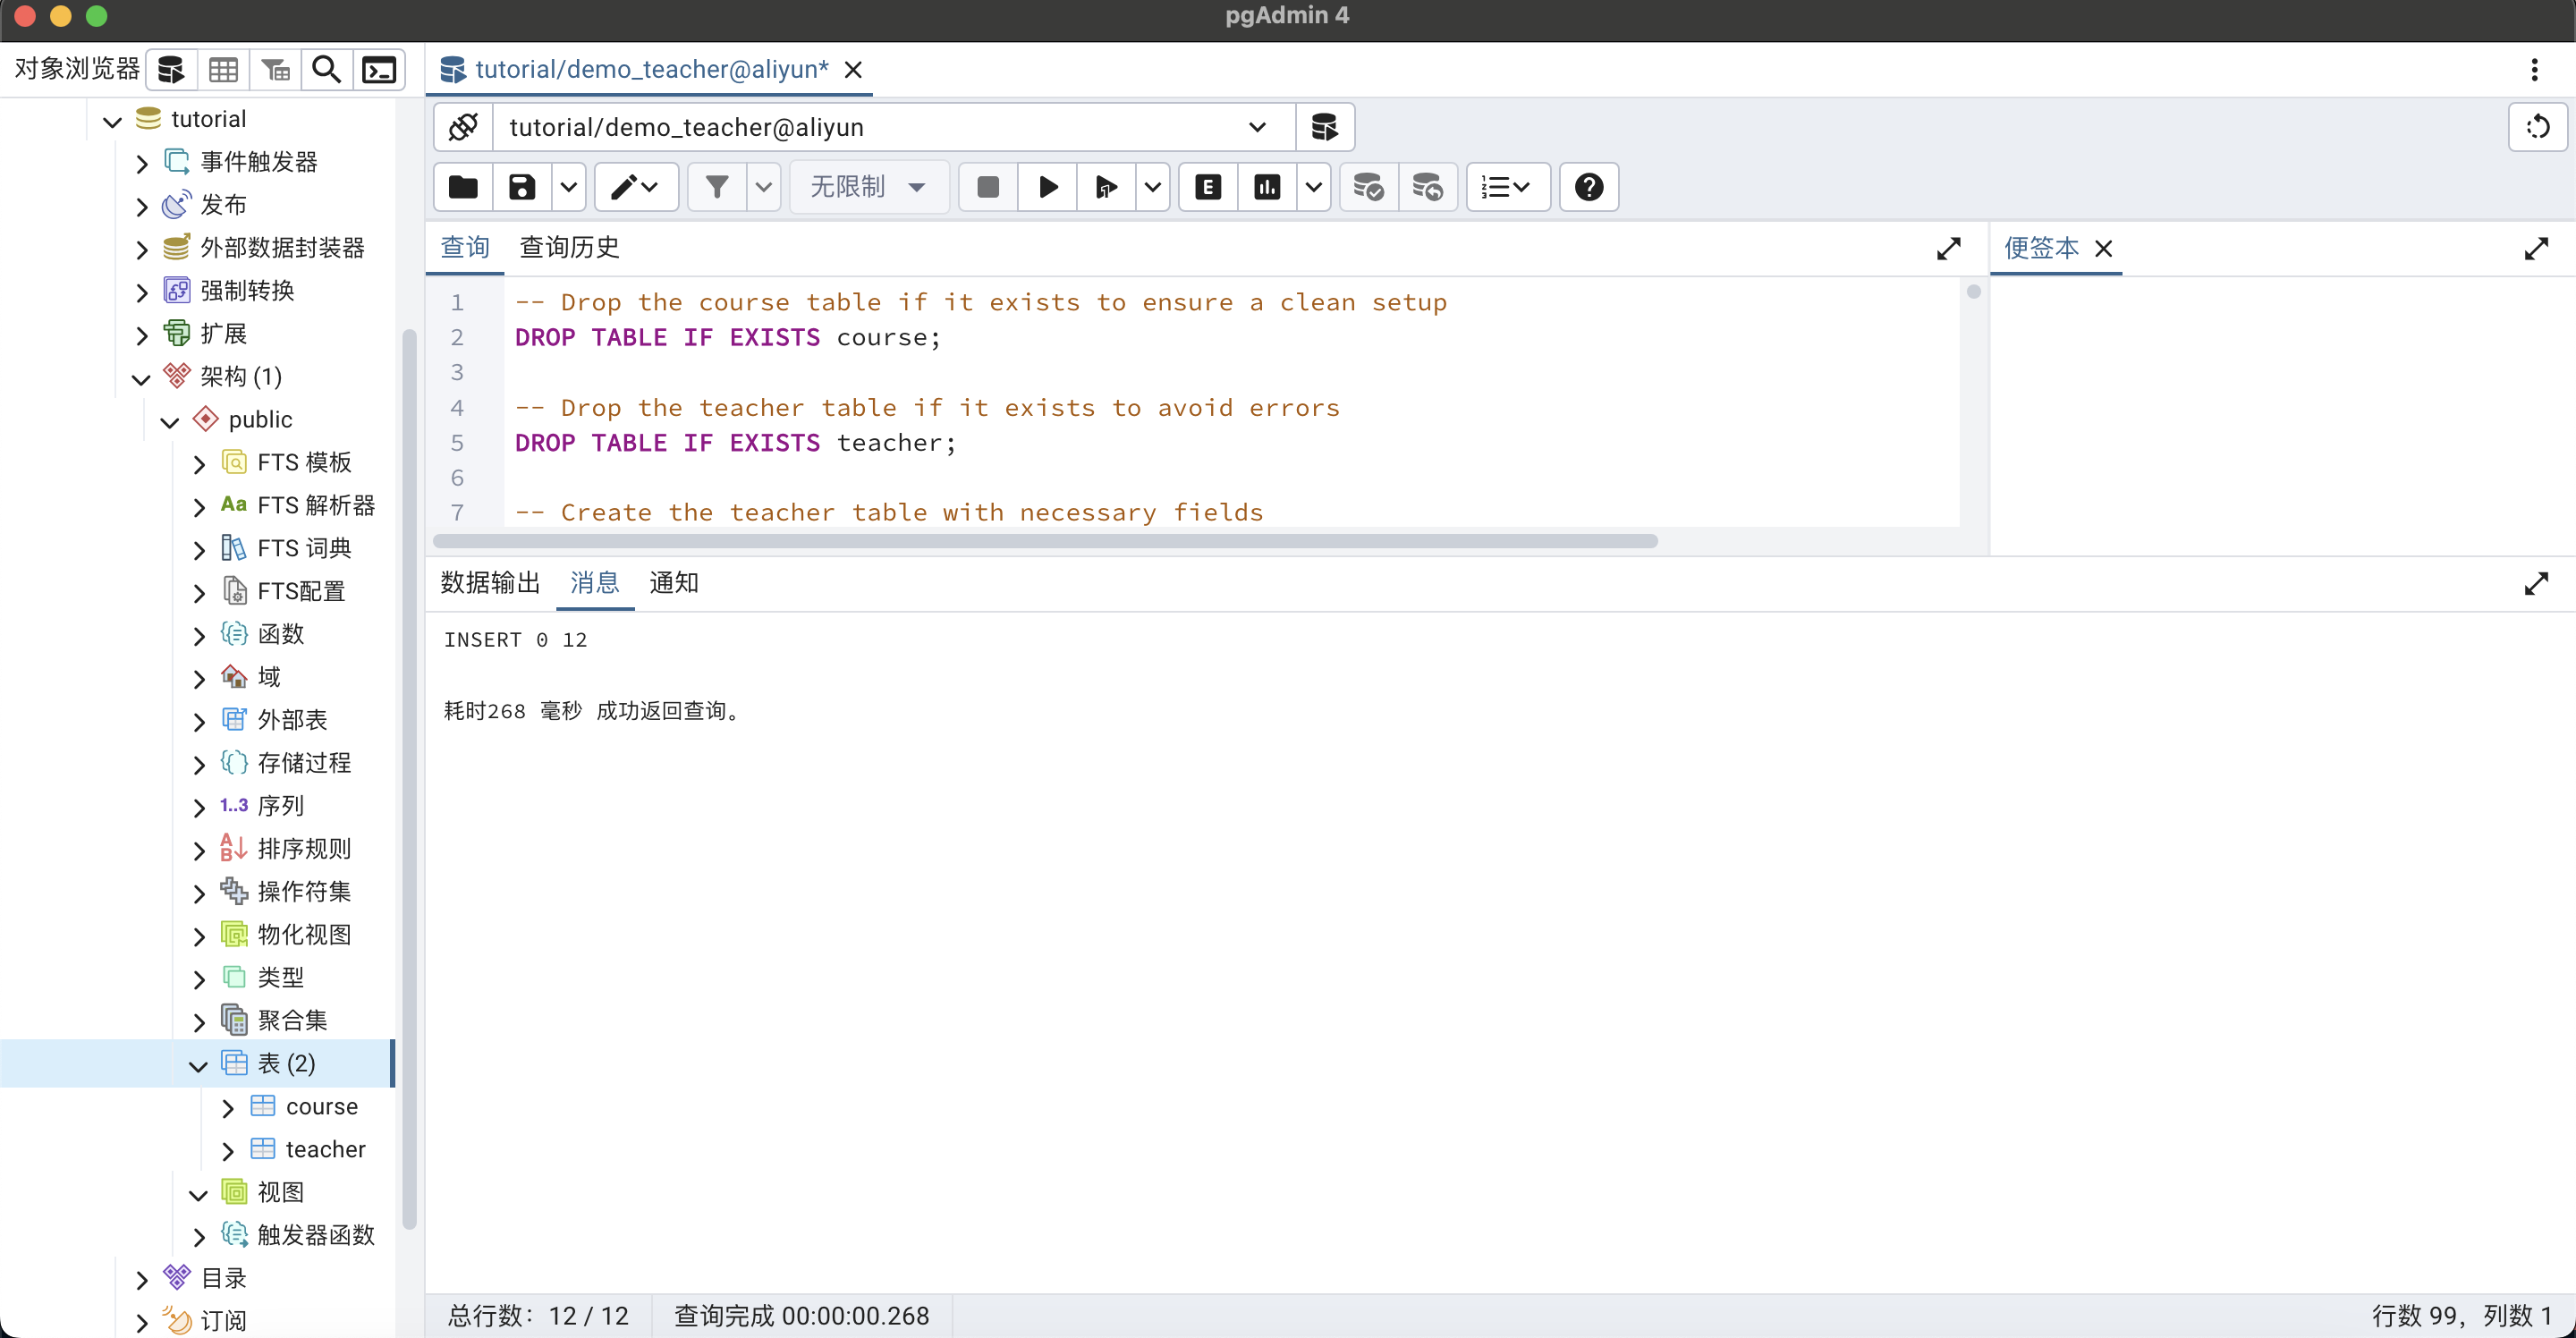
\includegraphics[width=13cm]{images/sec5/Init_DB.png}
\end{figure}

具体代码详见\hyperref[init_db]{附录}.

\subsection{后端设计}

后端主要分为课程管理与教师管理两个模块,具体框架如下图所示:
\begin{figure}[!htbp]
    \centering
    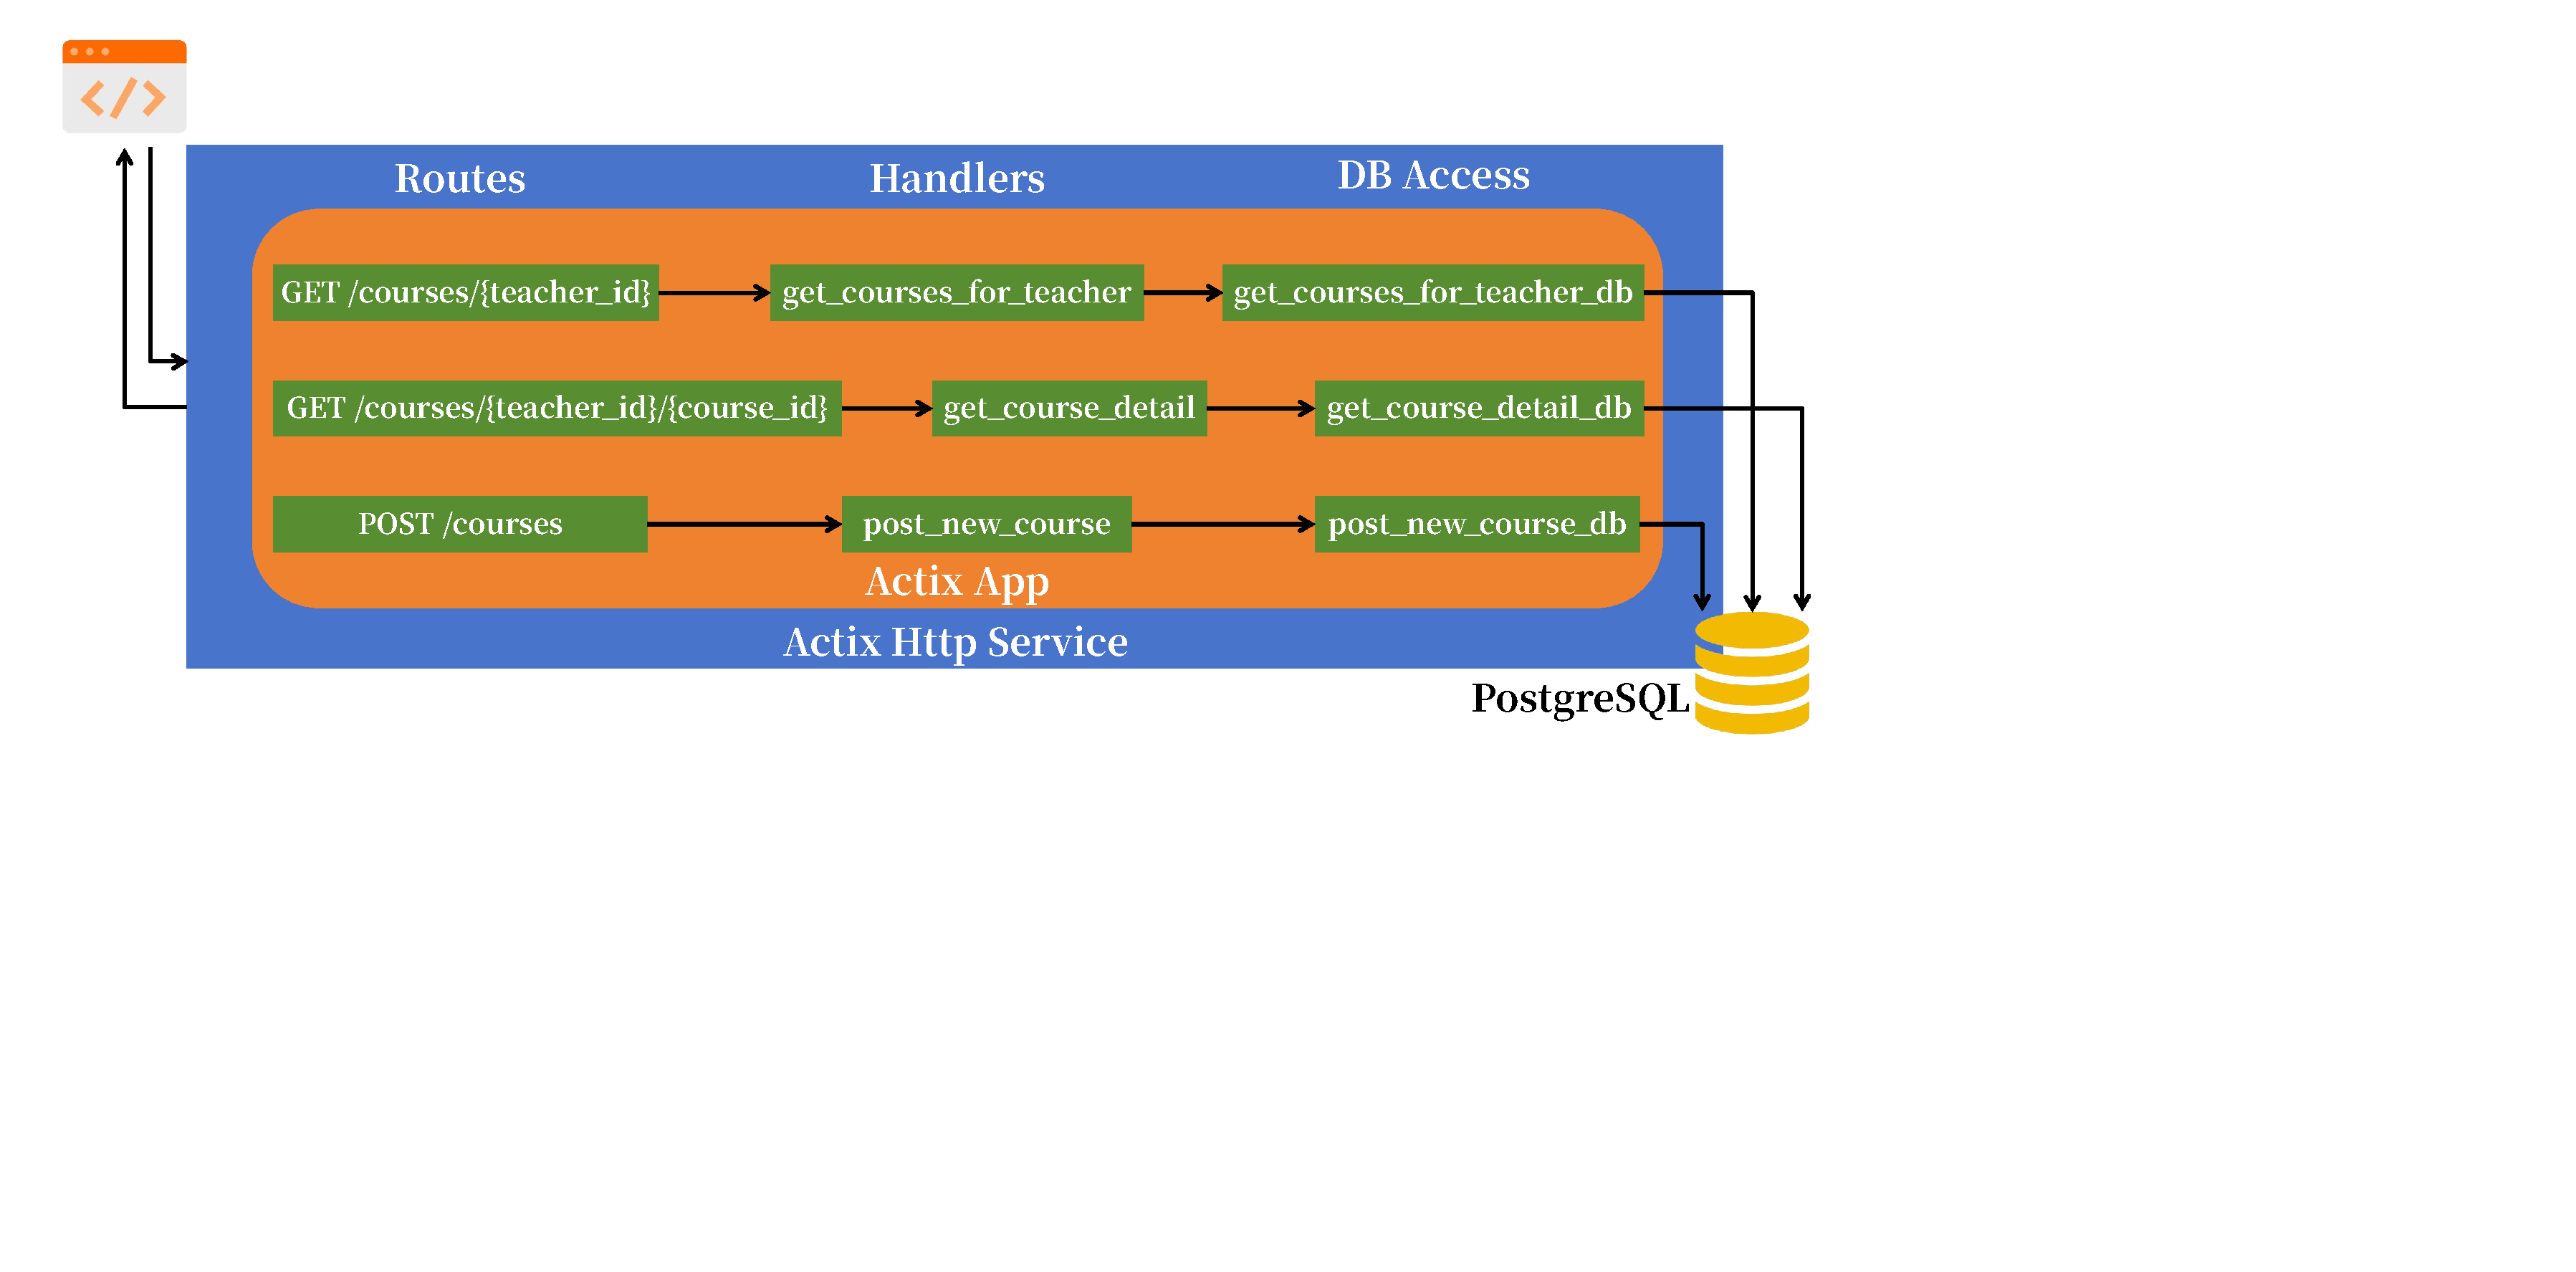
\includegraphics[width=13cm]{images/sec5/Back_End_Course.pdf}
    \caption{课程管理模块}
\end{figure}
\newpage
\begin{figure}[!htbp]
    \centering
    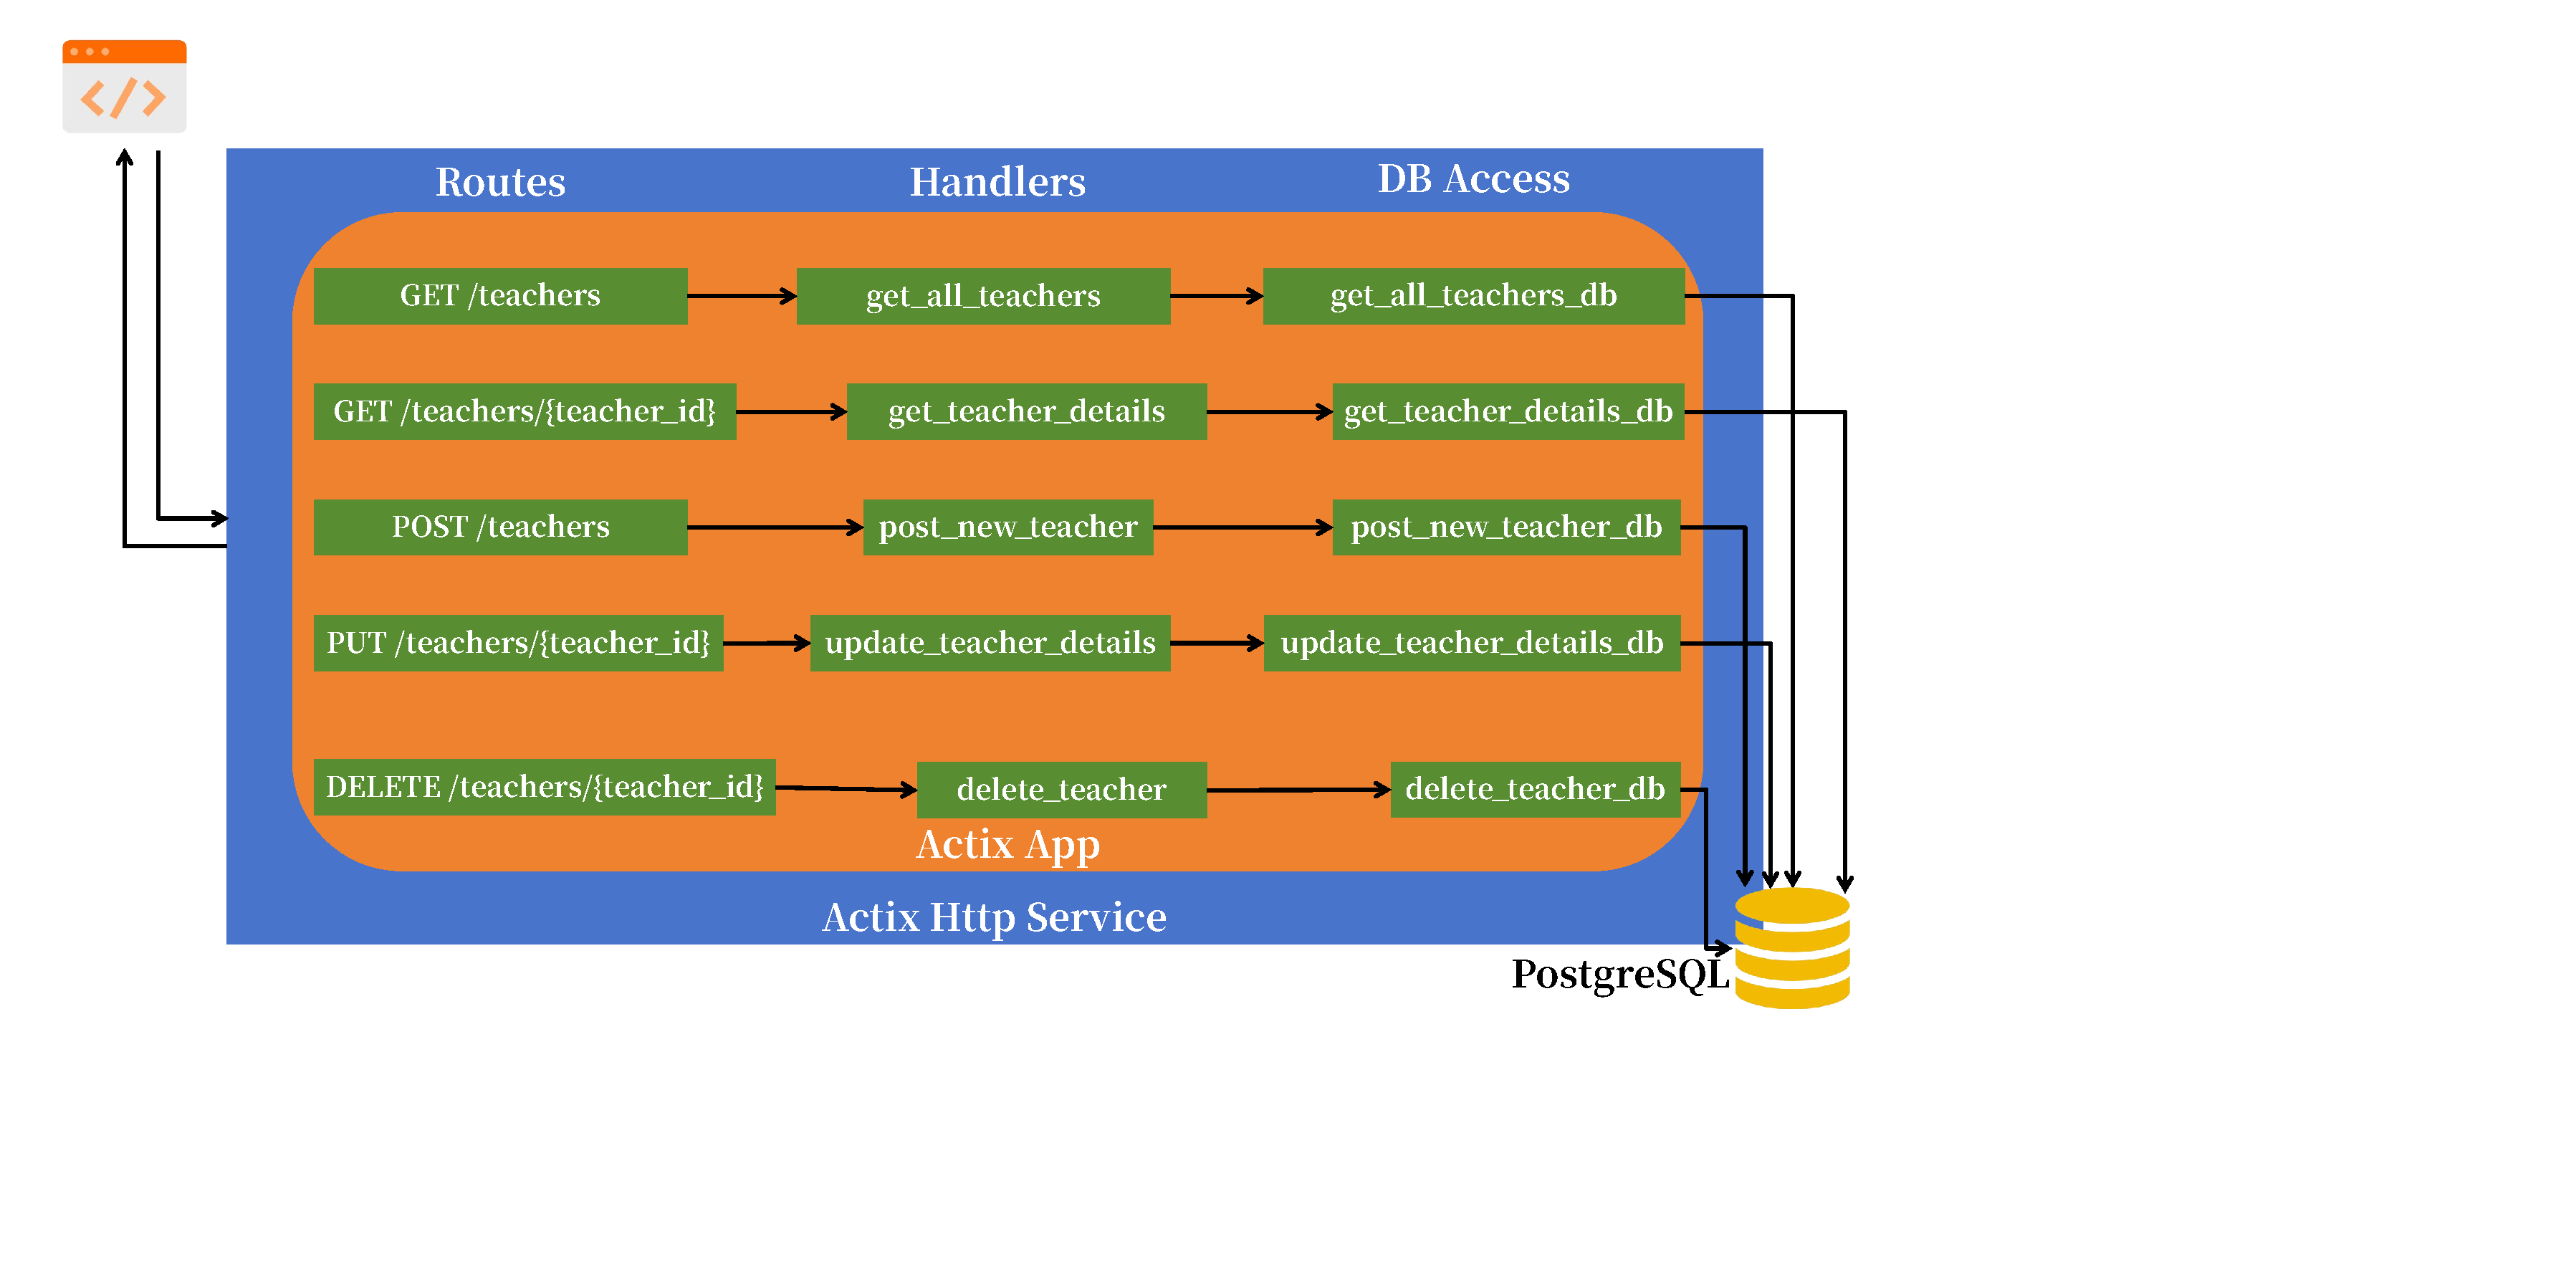
\includegraphics[width=13cm]{images/sec5/Back_End_Teacher.pdf}
    \caption{教师管理模块}
\end{figure}

同时自行编写错误类型与处理函数,具体框架如下图所示:
\begin{figure}[!htbp]
    \centering
    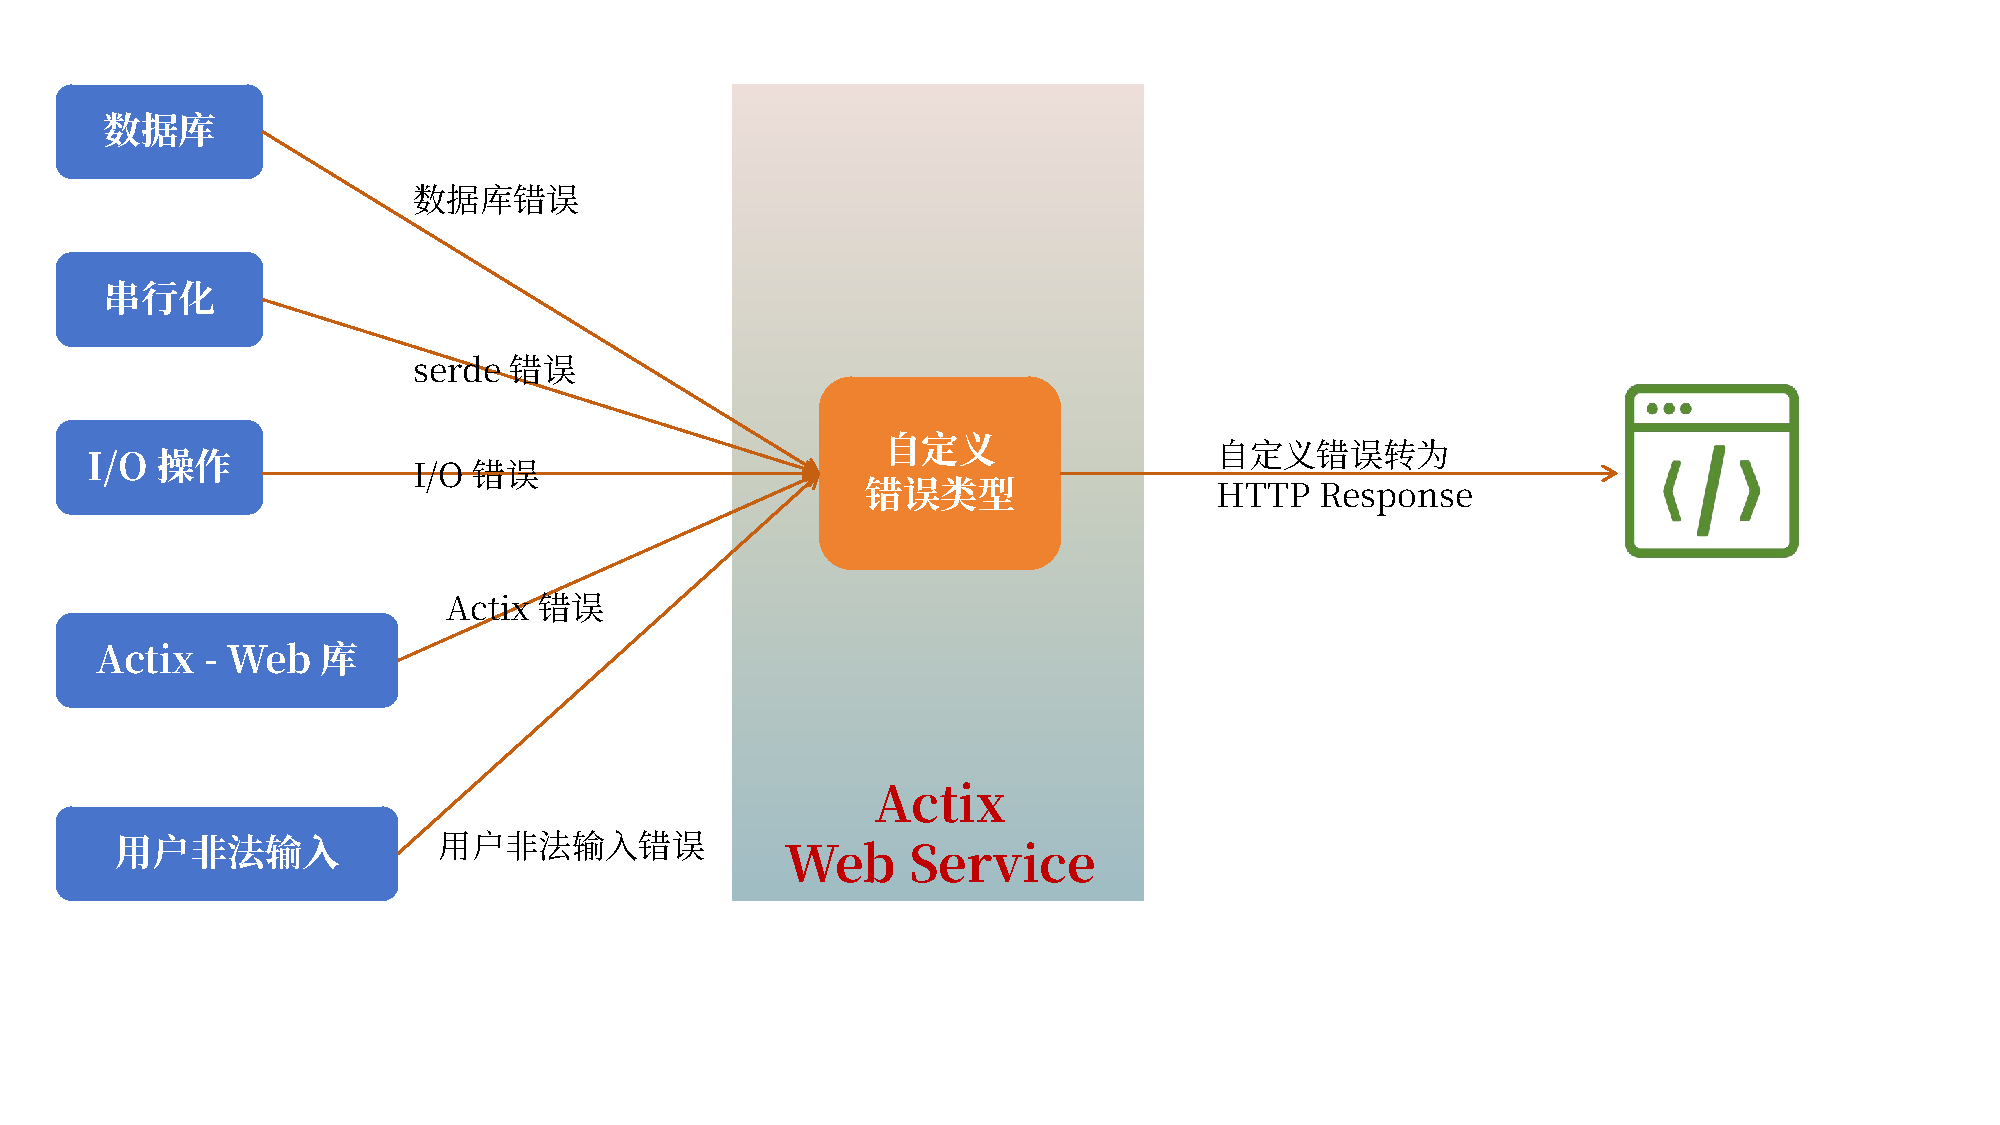
\includegraphics[width=13cm]{images/sec5/My_Error.pdf}
    \caption{错误处理模块}
\end{figure}

最后,启动 Web 服务,发布到端口 3000:
\begin{figure}[!htbp]
    \centering
    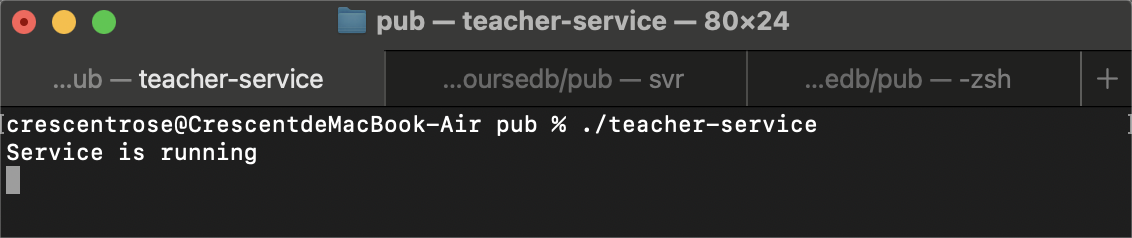
\includegraphics[width=13cm]{images/sec5/teacher-service.png}
\end{figure}

\subsection{前端设计}

在前端部分,我使用 Rust 模板引擎 \href{https://keats.github.io/tera/}{Tera} 构建教师管理模块的前端页面;同时使用 \href{https://www.rust-lang.org/what/wasm}{Web­Assembly} 构建课程管理模块的前端页面. 整个系统的具体框架如下图所示:
\begin{figure}[!htbp]
    \centering
    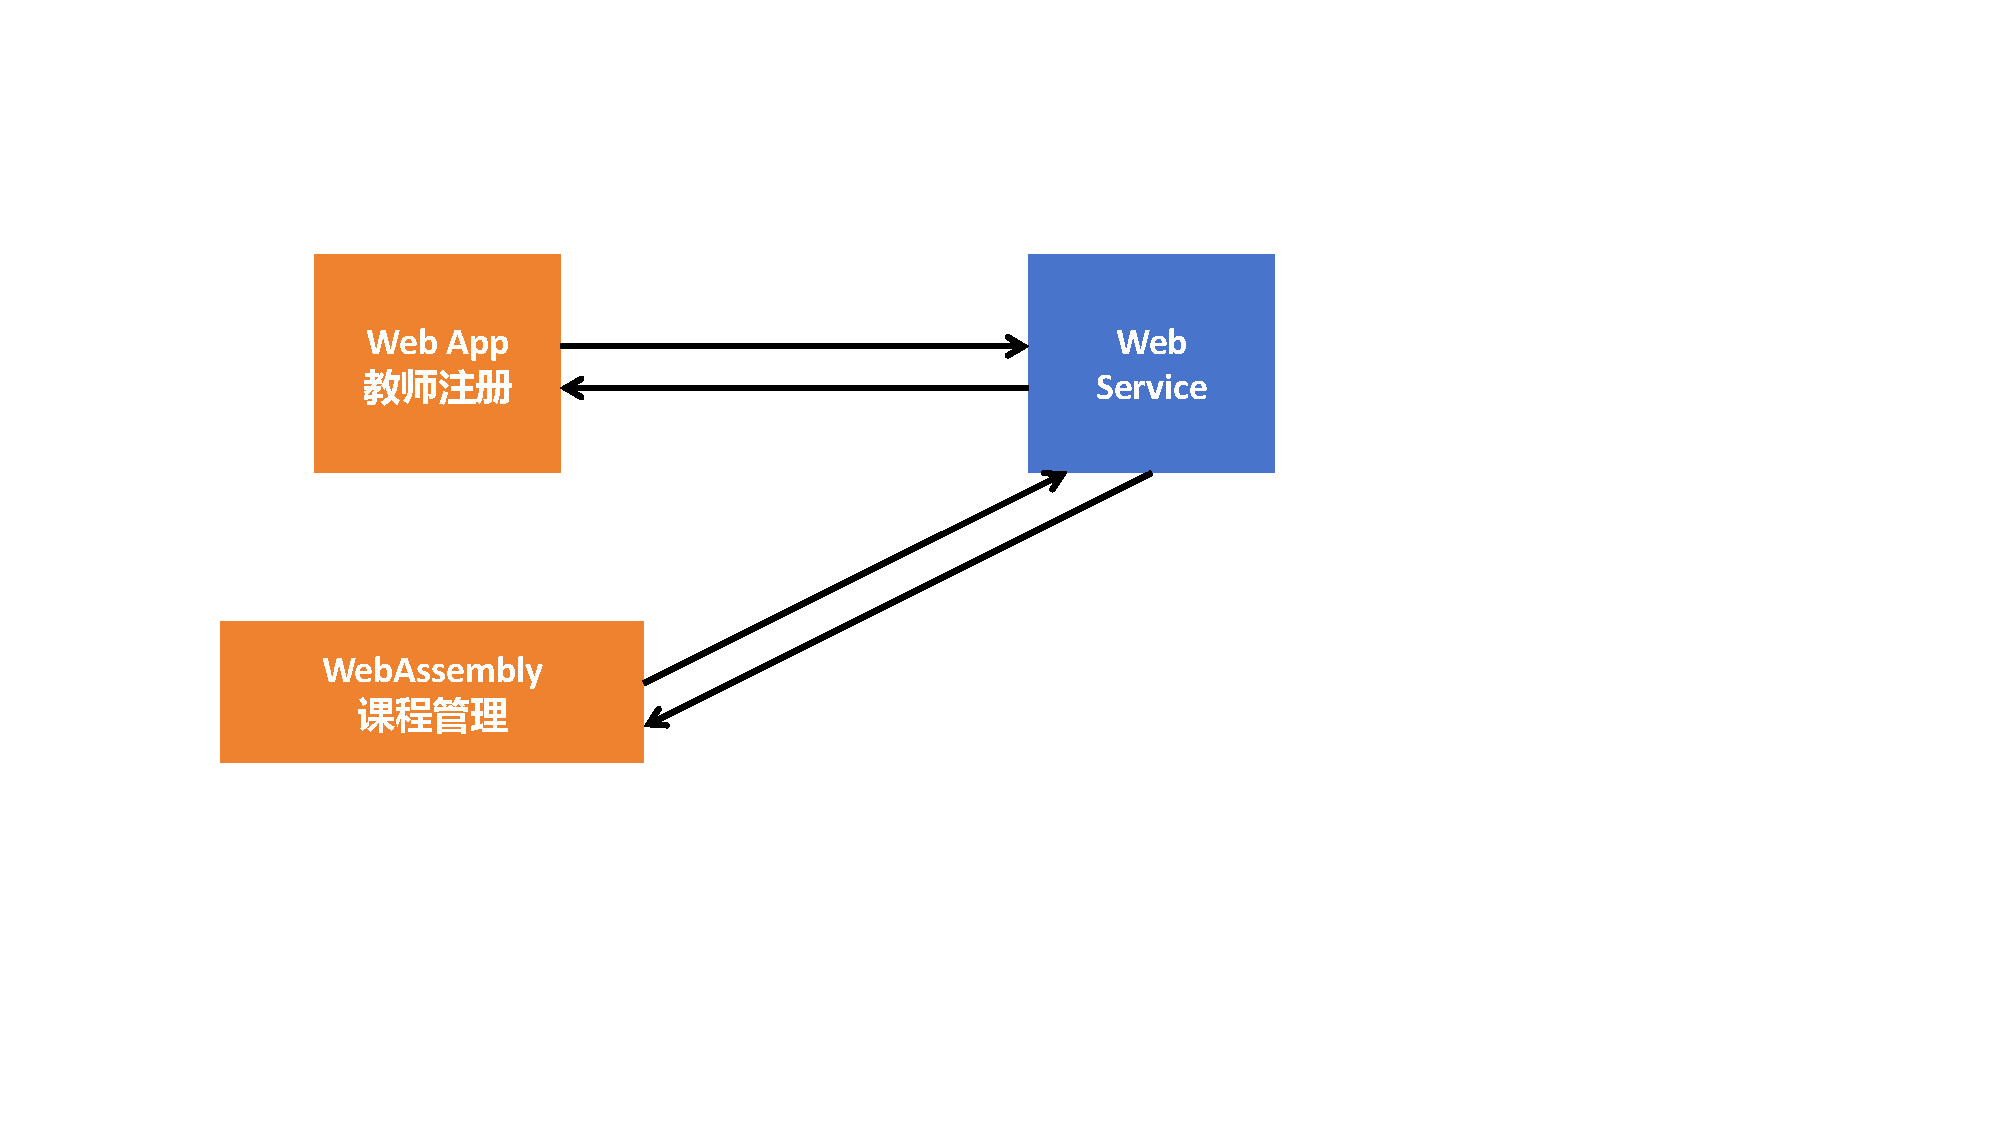
\includegraphics[width=13cm]{images/sec5/Framework.pdf}
    \caption{系统框架}
\end{figure}

\subsubsection{教师管理模块}
首先启动 Web App,监听端口 3000 并渲染教师管理页面,发布到端口 8080:
\begin{figure}[!htbp]
    \centering
    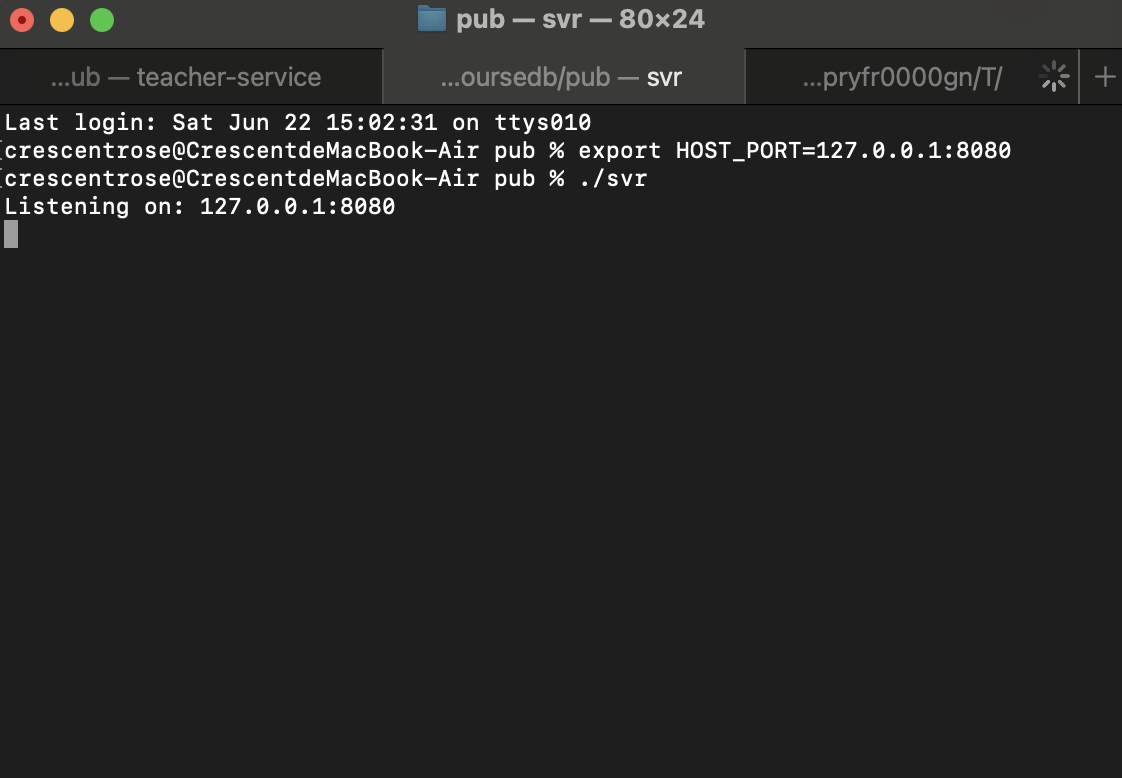
\includegraphics[width=13cm]{images/sec5/svr.png}
\end{figure}
\newpage
接着打开本地浏览器,访问 \texttt{http://localhost:8080},即可看到教师管理页面:
\begin{figure}[!htbp]
    \centering
    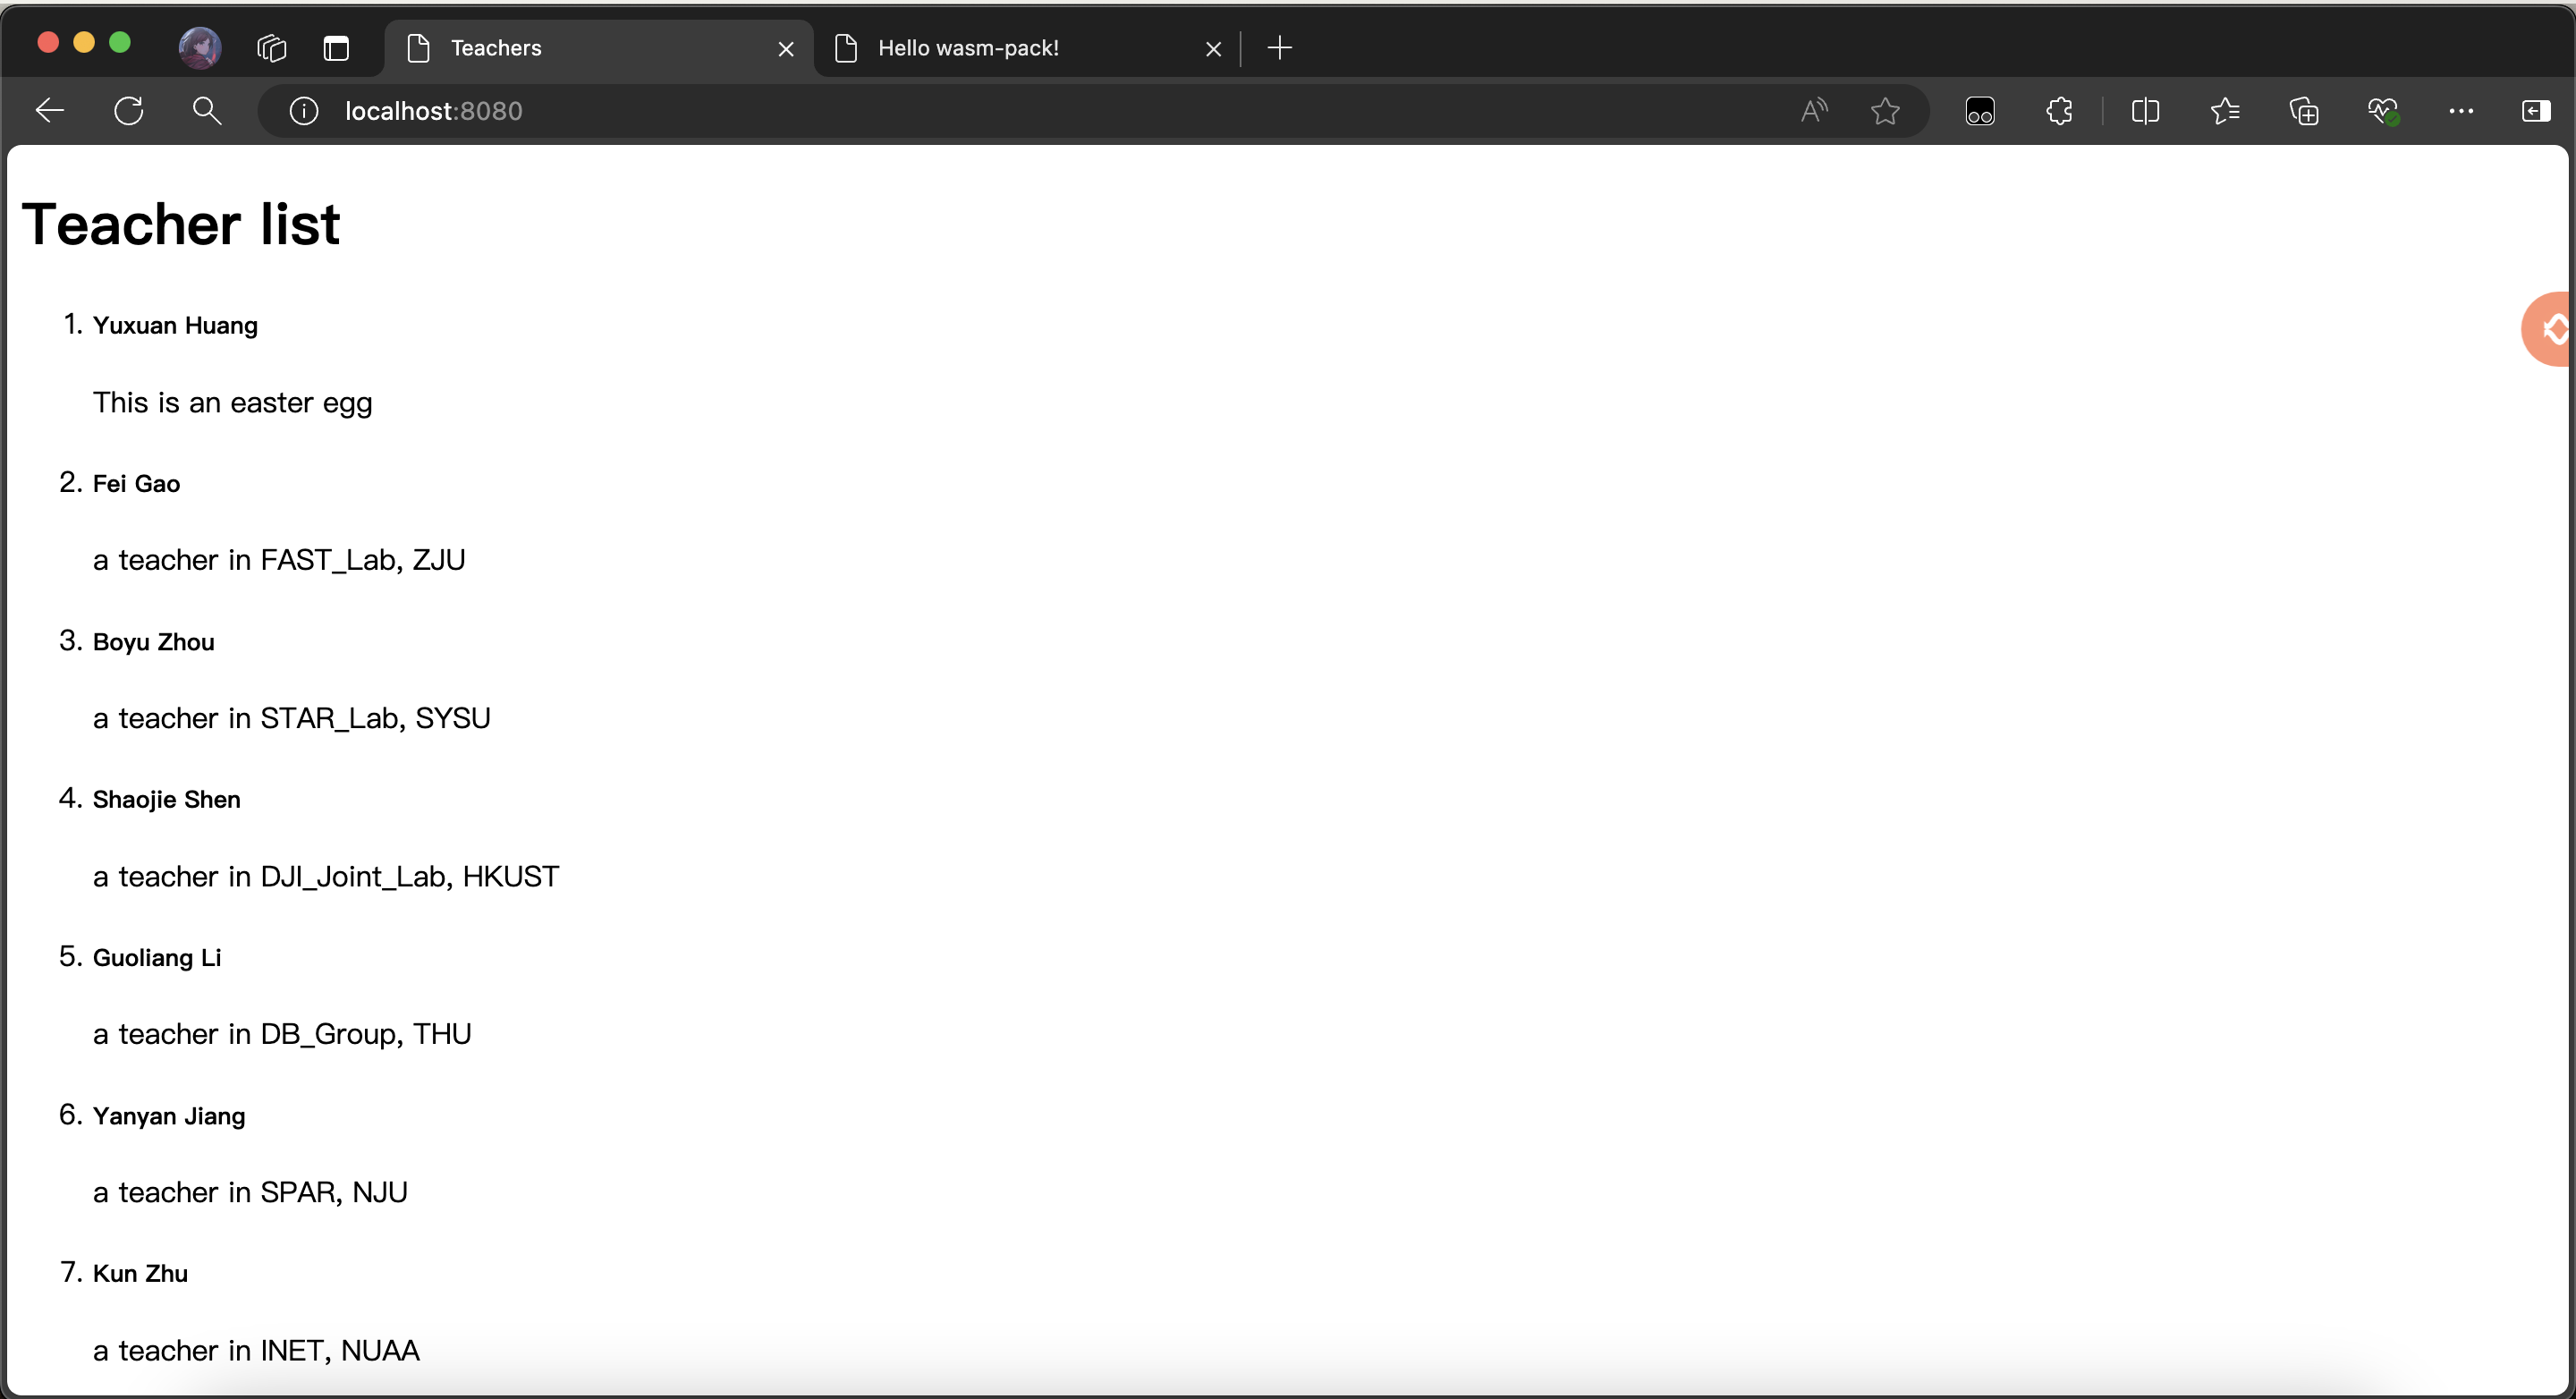
\includegraphics[width=13cm]{images/sec5/Teacher_Manage_Page.png}
\end{figure}

点击底部的 \texttt{Register a teacher} 按钮,即可进入教师注册页面:
\begin{figure}[!htbp]
    \centering
    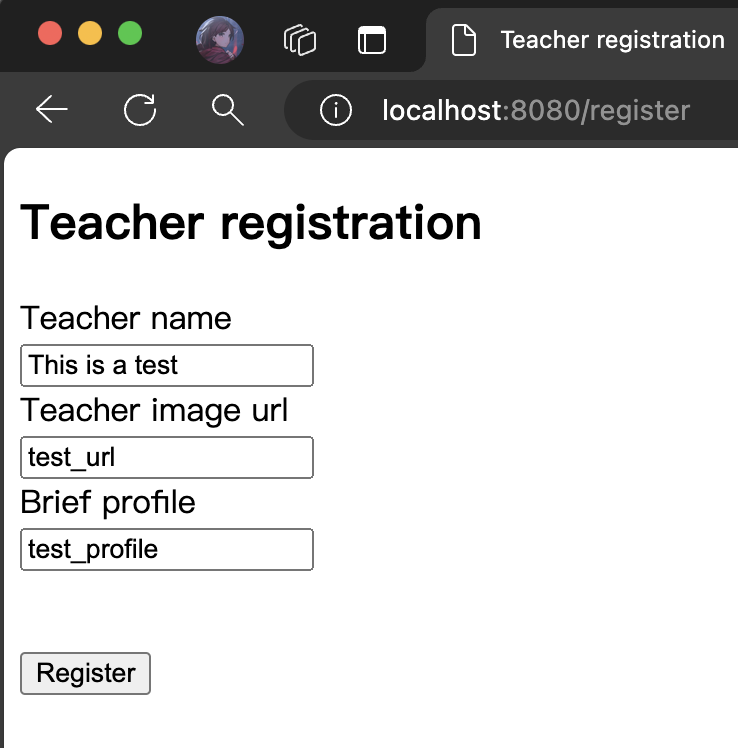
\includegraphics[width=13cm]{images/sec5/Add_Teacher.png}
\end{figure}

点击底部的 \texttt{Register} 按钮,即可成功添加:
\begin{figure}[!htbp]
    \centering
    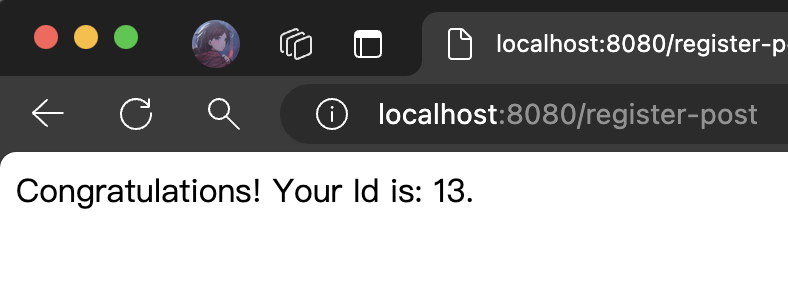
\includegraphics[width=13cm]{images/sec5/Add_Teacher_Success.png}
\end{figure}

返回教师管理页面,可以看到添加的教师信息:
\begin{figure}[!htbp]
    \centering
    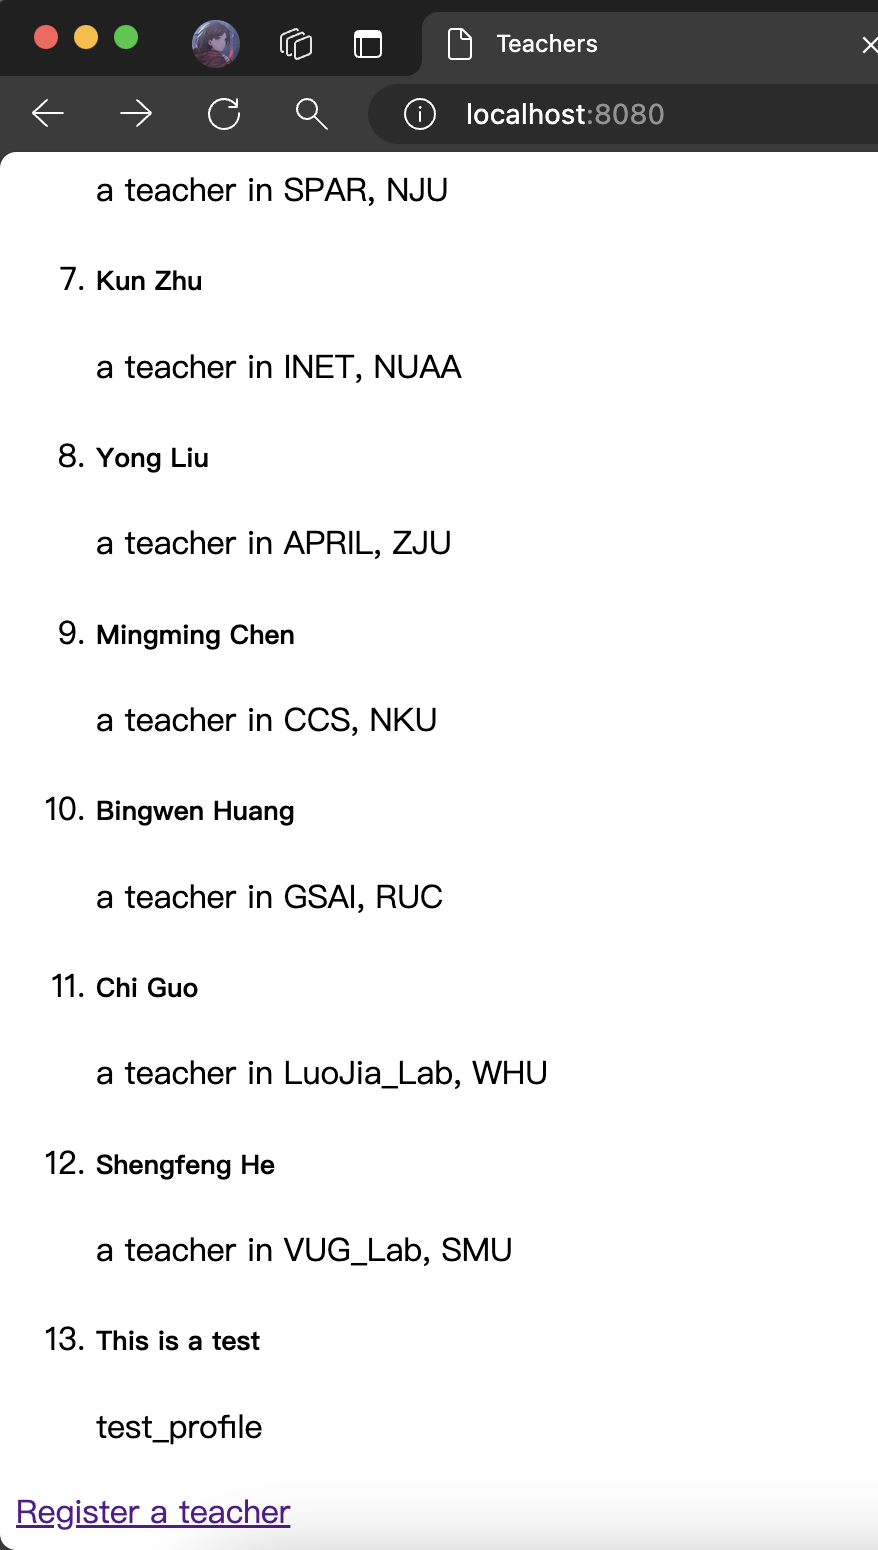
\includegraphics[width=8cm]{images/sec5/Add_Teacher_Check.png}
\end{figure}

\subsubsection{课程管理模块}

首先启动 Wasm-client,监听端口 3000 并渲染课程管理页面,发布到端口 8081:
\begin{figure}[!htbp]
    \centering
    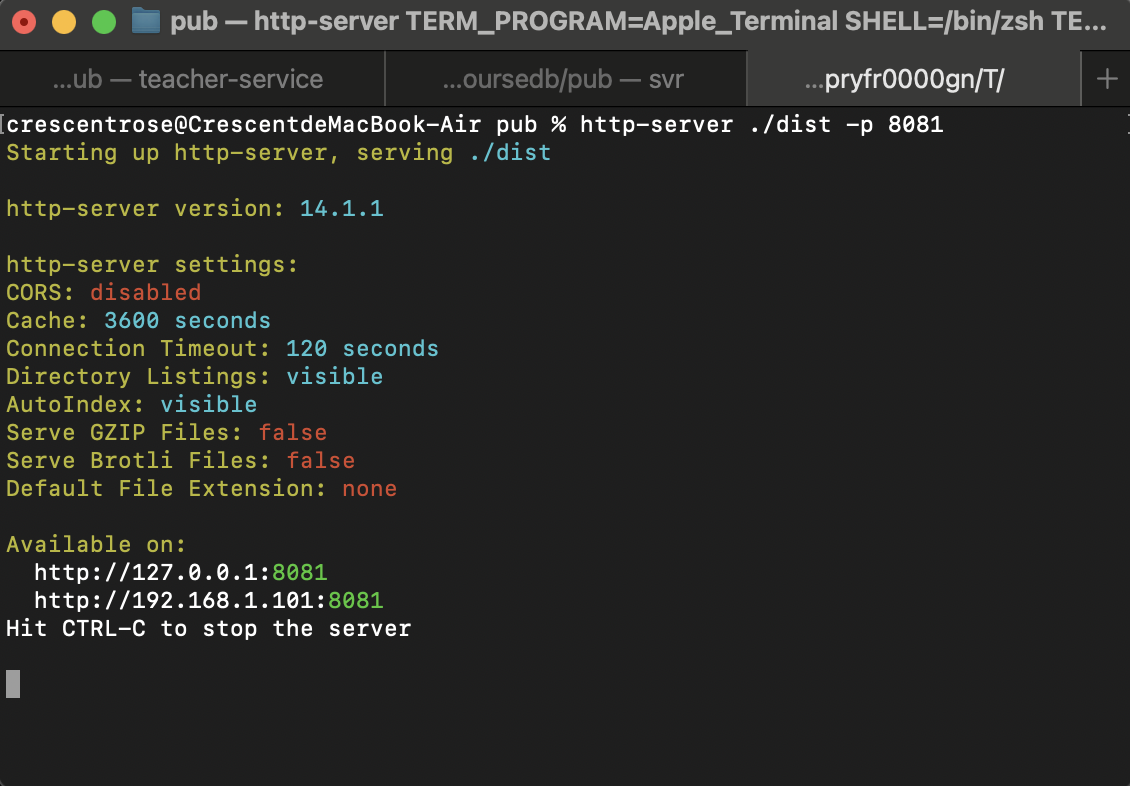
\includegraphics[width=13cm]{images/sec5/wasm.png}
\end{figure}

接着打开本地浏览器,访问 \texttt{http://localhost:8081},即可看到课程管理页面:
\begin{figure}[!htbp]
    \centering
    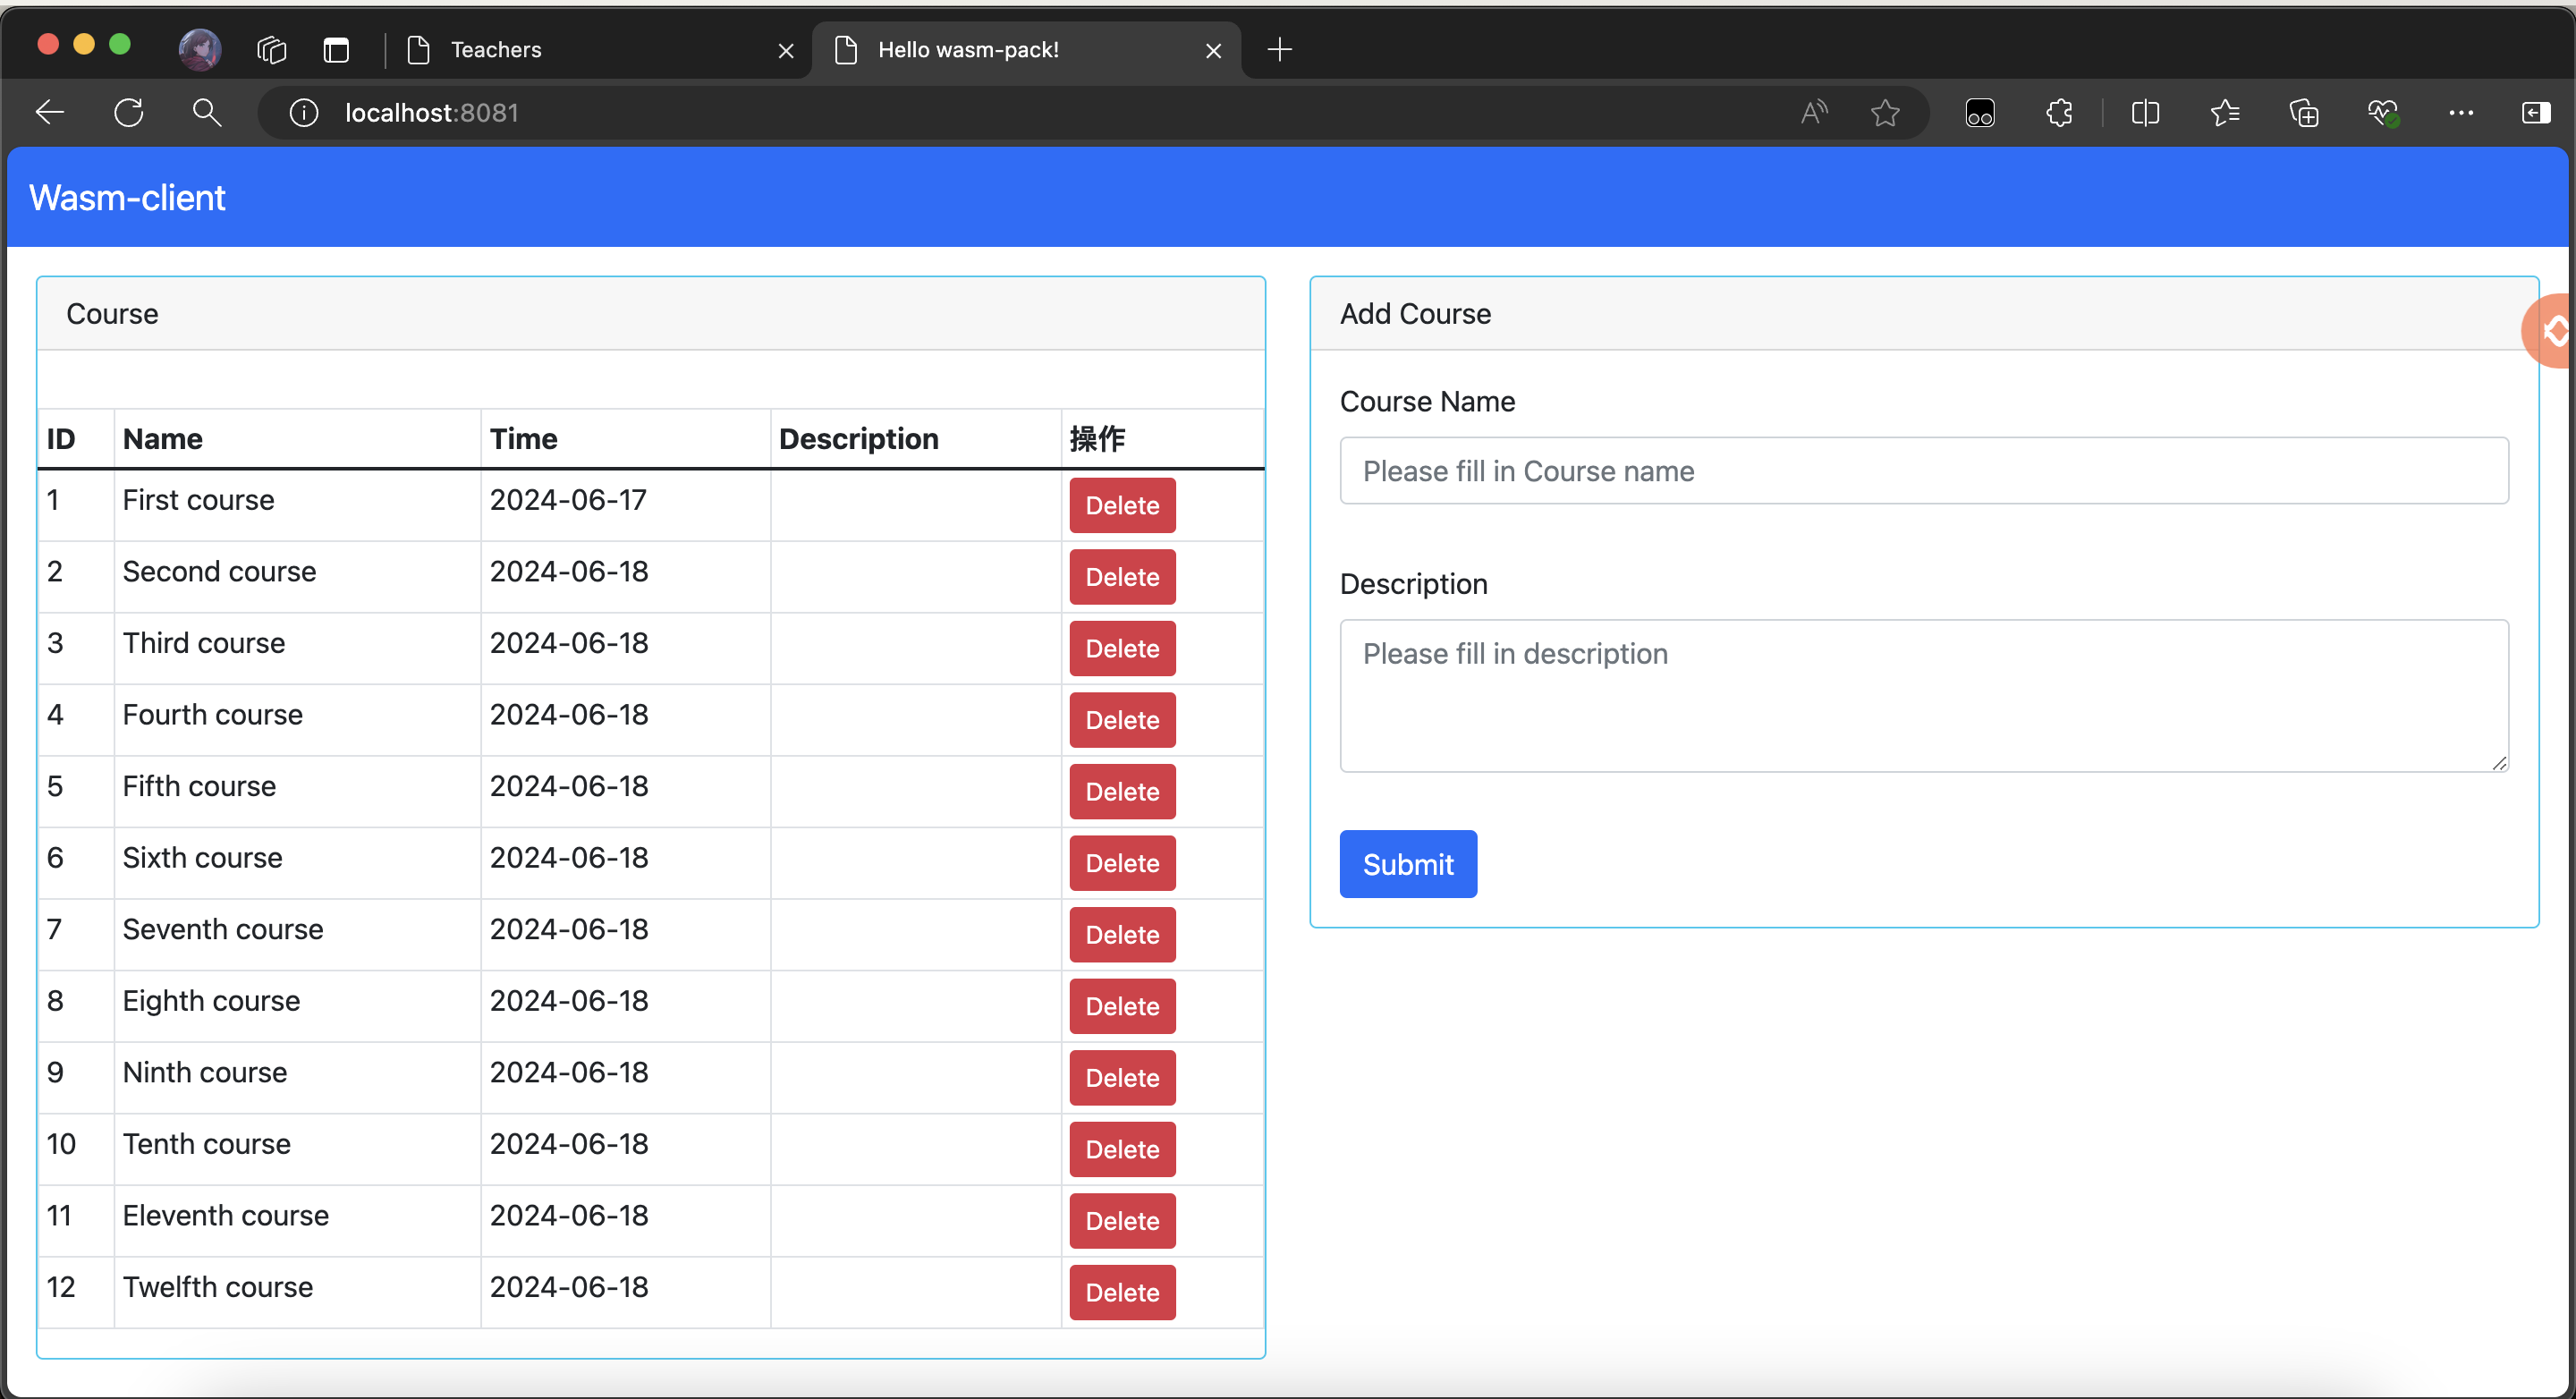
\includegraphics[width=13cm]{images/sec5/Course_Manage_Page.png}
\end{figure}
\newpage
在右边的窗口中输入课程信息,点击 \texttt{Submit} 按钮,即可添加课程:
\begin{figure}[!htbp]
    \centering
    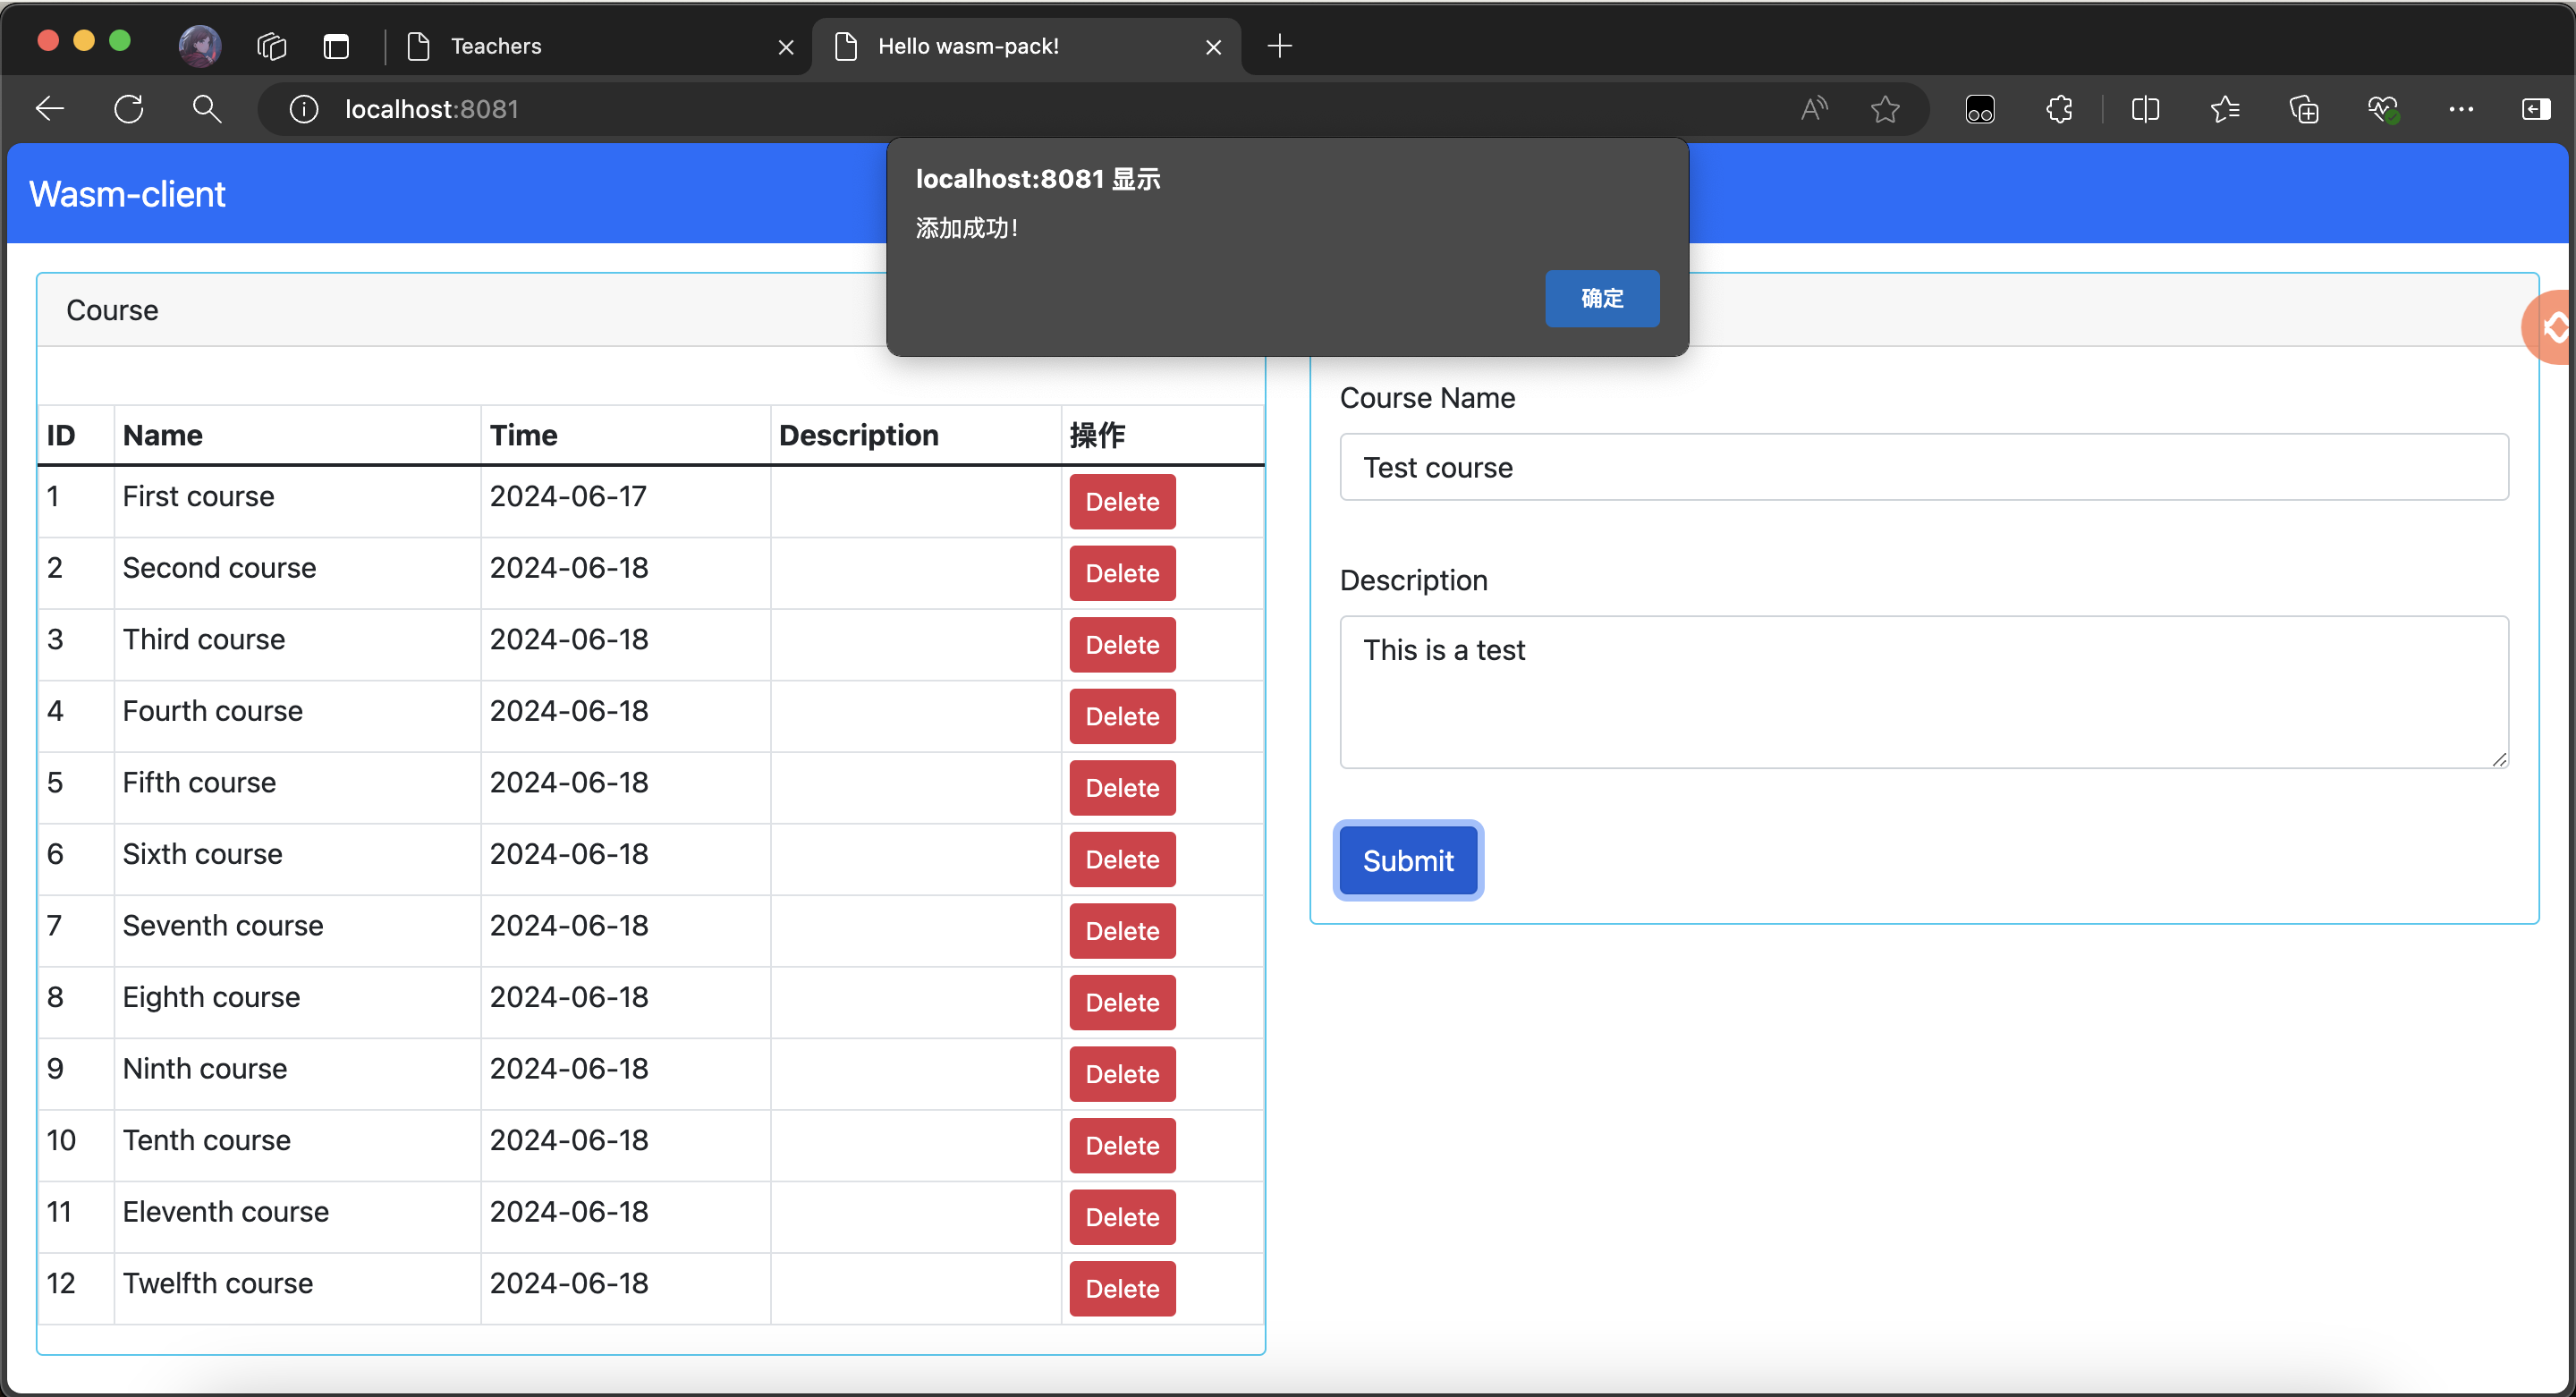
\includegraphics[width=13cm]{images/sec5/Add_Course.png}
\end{figure}

返回课程管理页面,可以看到添加的课程信息:
\begin{figure}[!htbp]
    \centering
    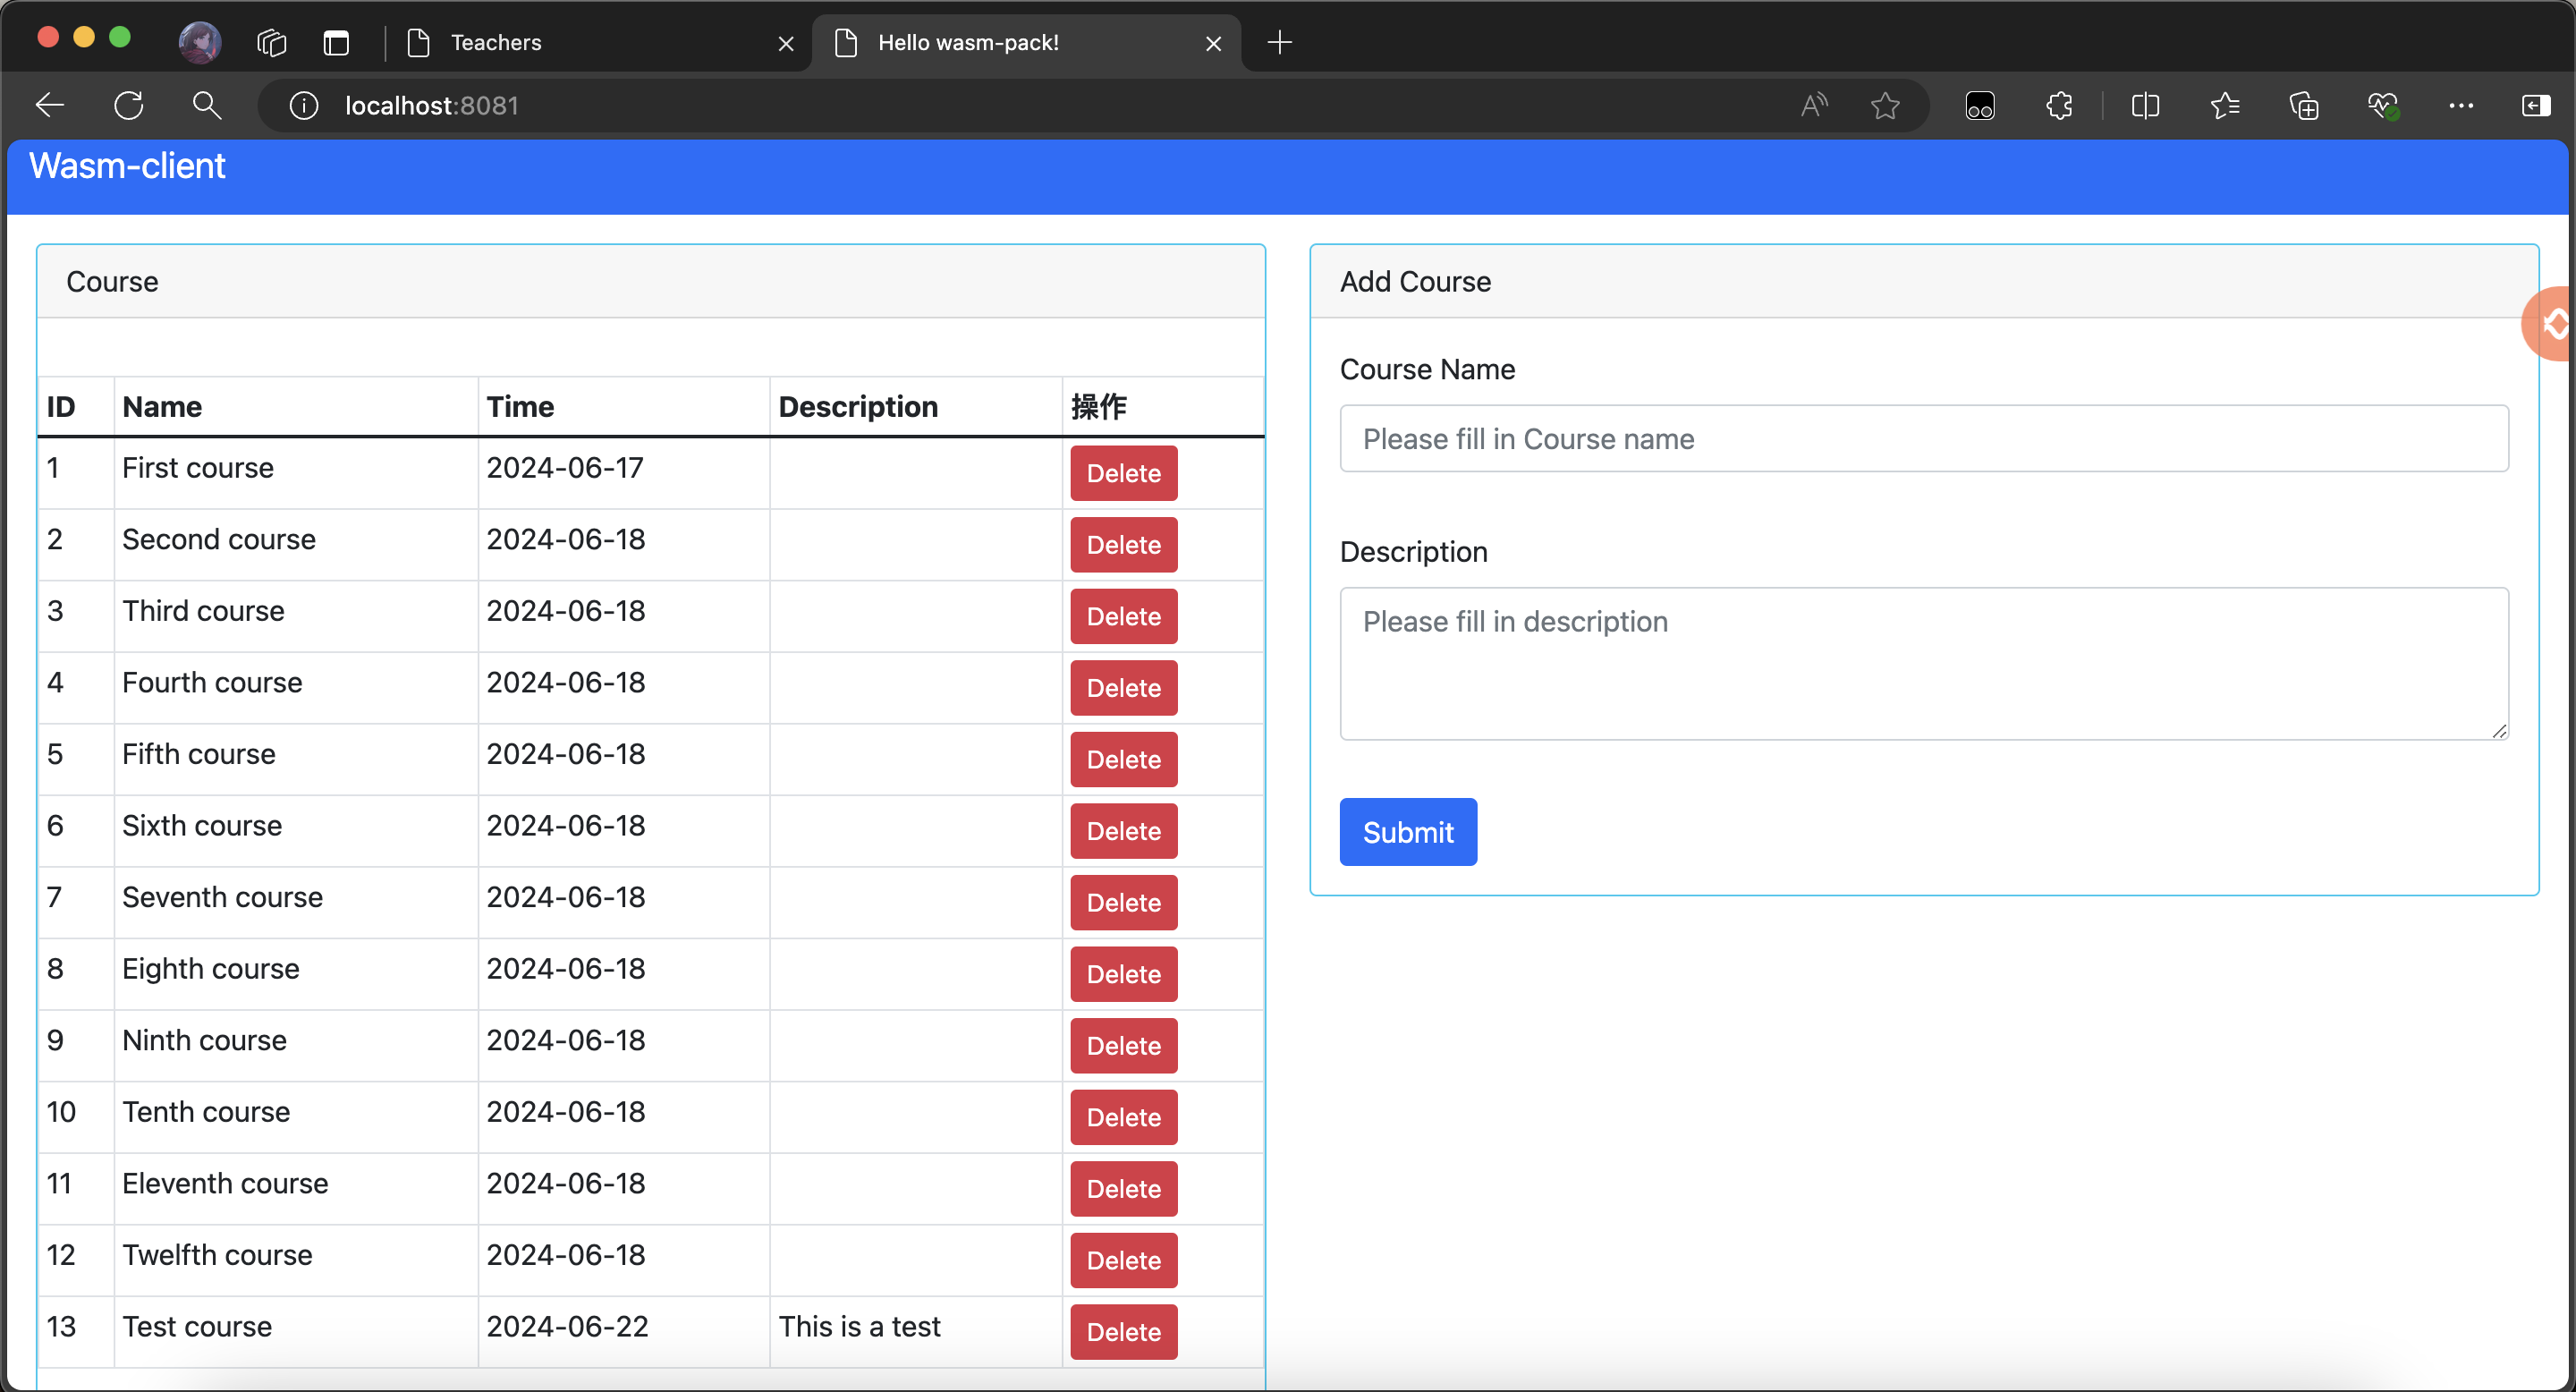
\includegraphics[width=13cm]{images/sec5/Add_Course_Success.png}
\end{figure}
\newpage
在左边的窗口选择你想要删除的课程,点击 \texttt{Delete} 按钮,会弹出确认框,点击 \texttt{确定} 即可删除:
\begin{figure}[!htbp]
    \centering
    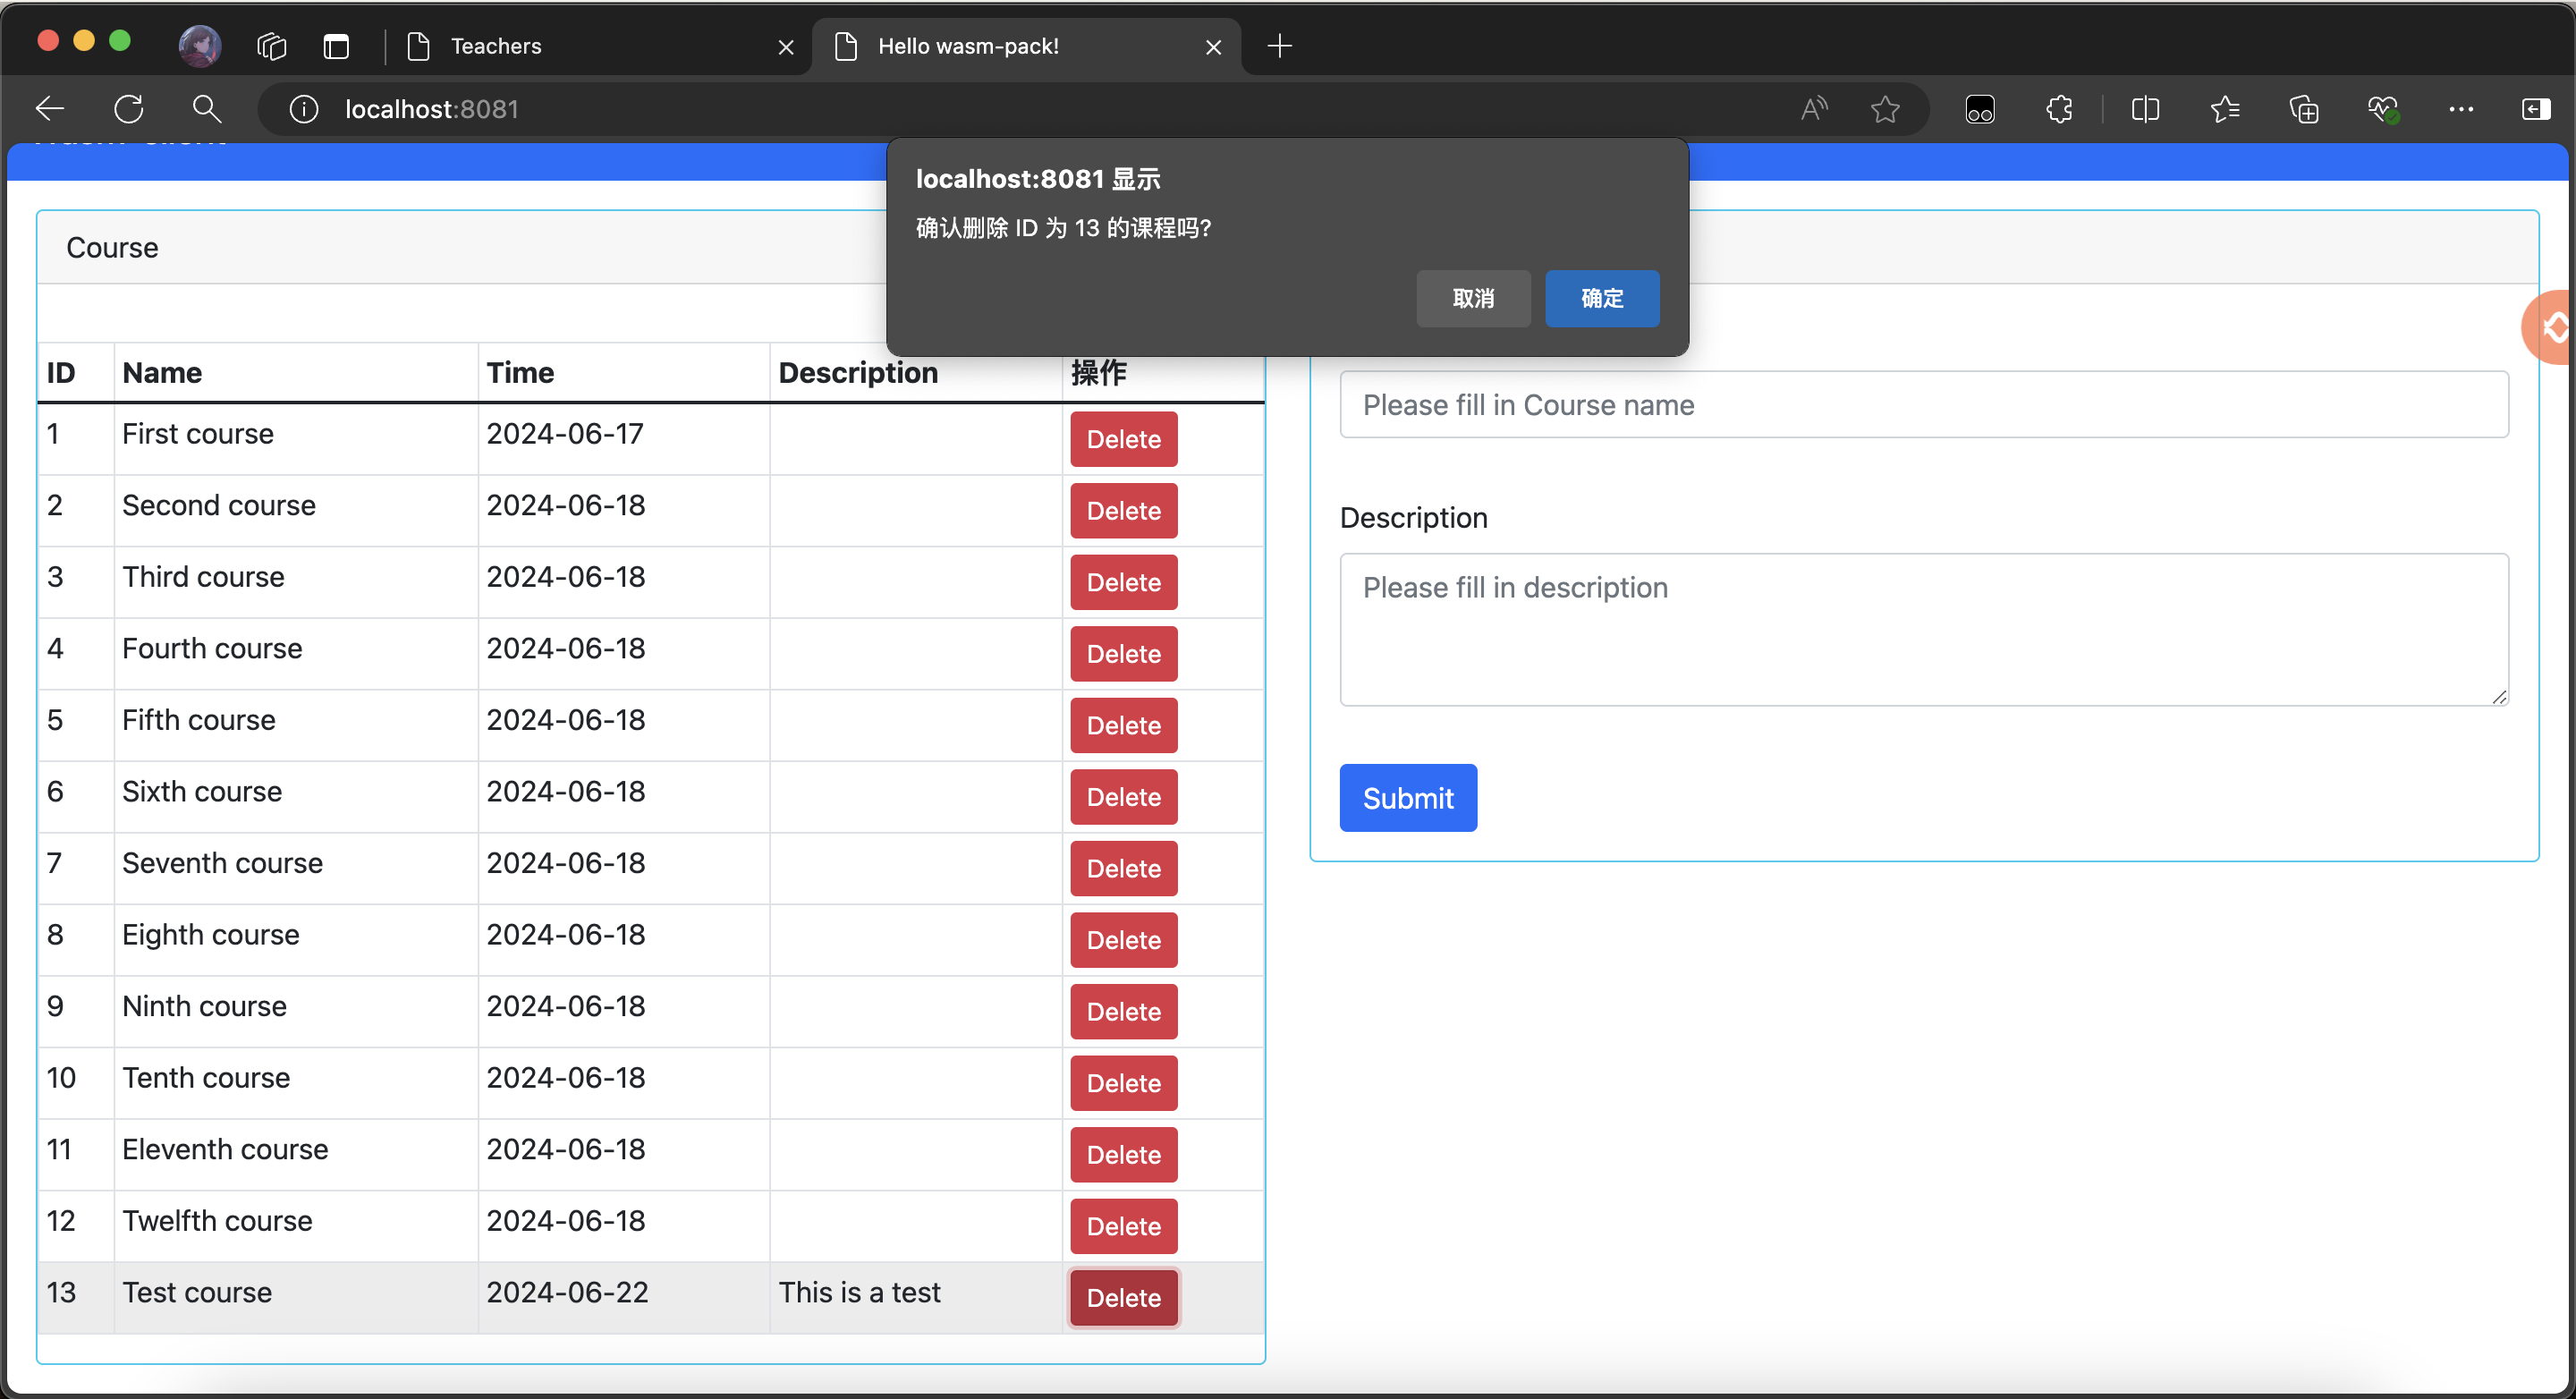
\includegraphics[width=13cm]{images/sec5/Delete_Course.png}
\end{figure}

弹出窗口提示删除成功:
\begin{figure}[!htbp]
    \centering
    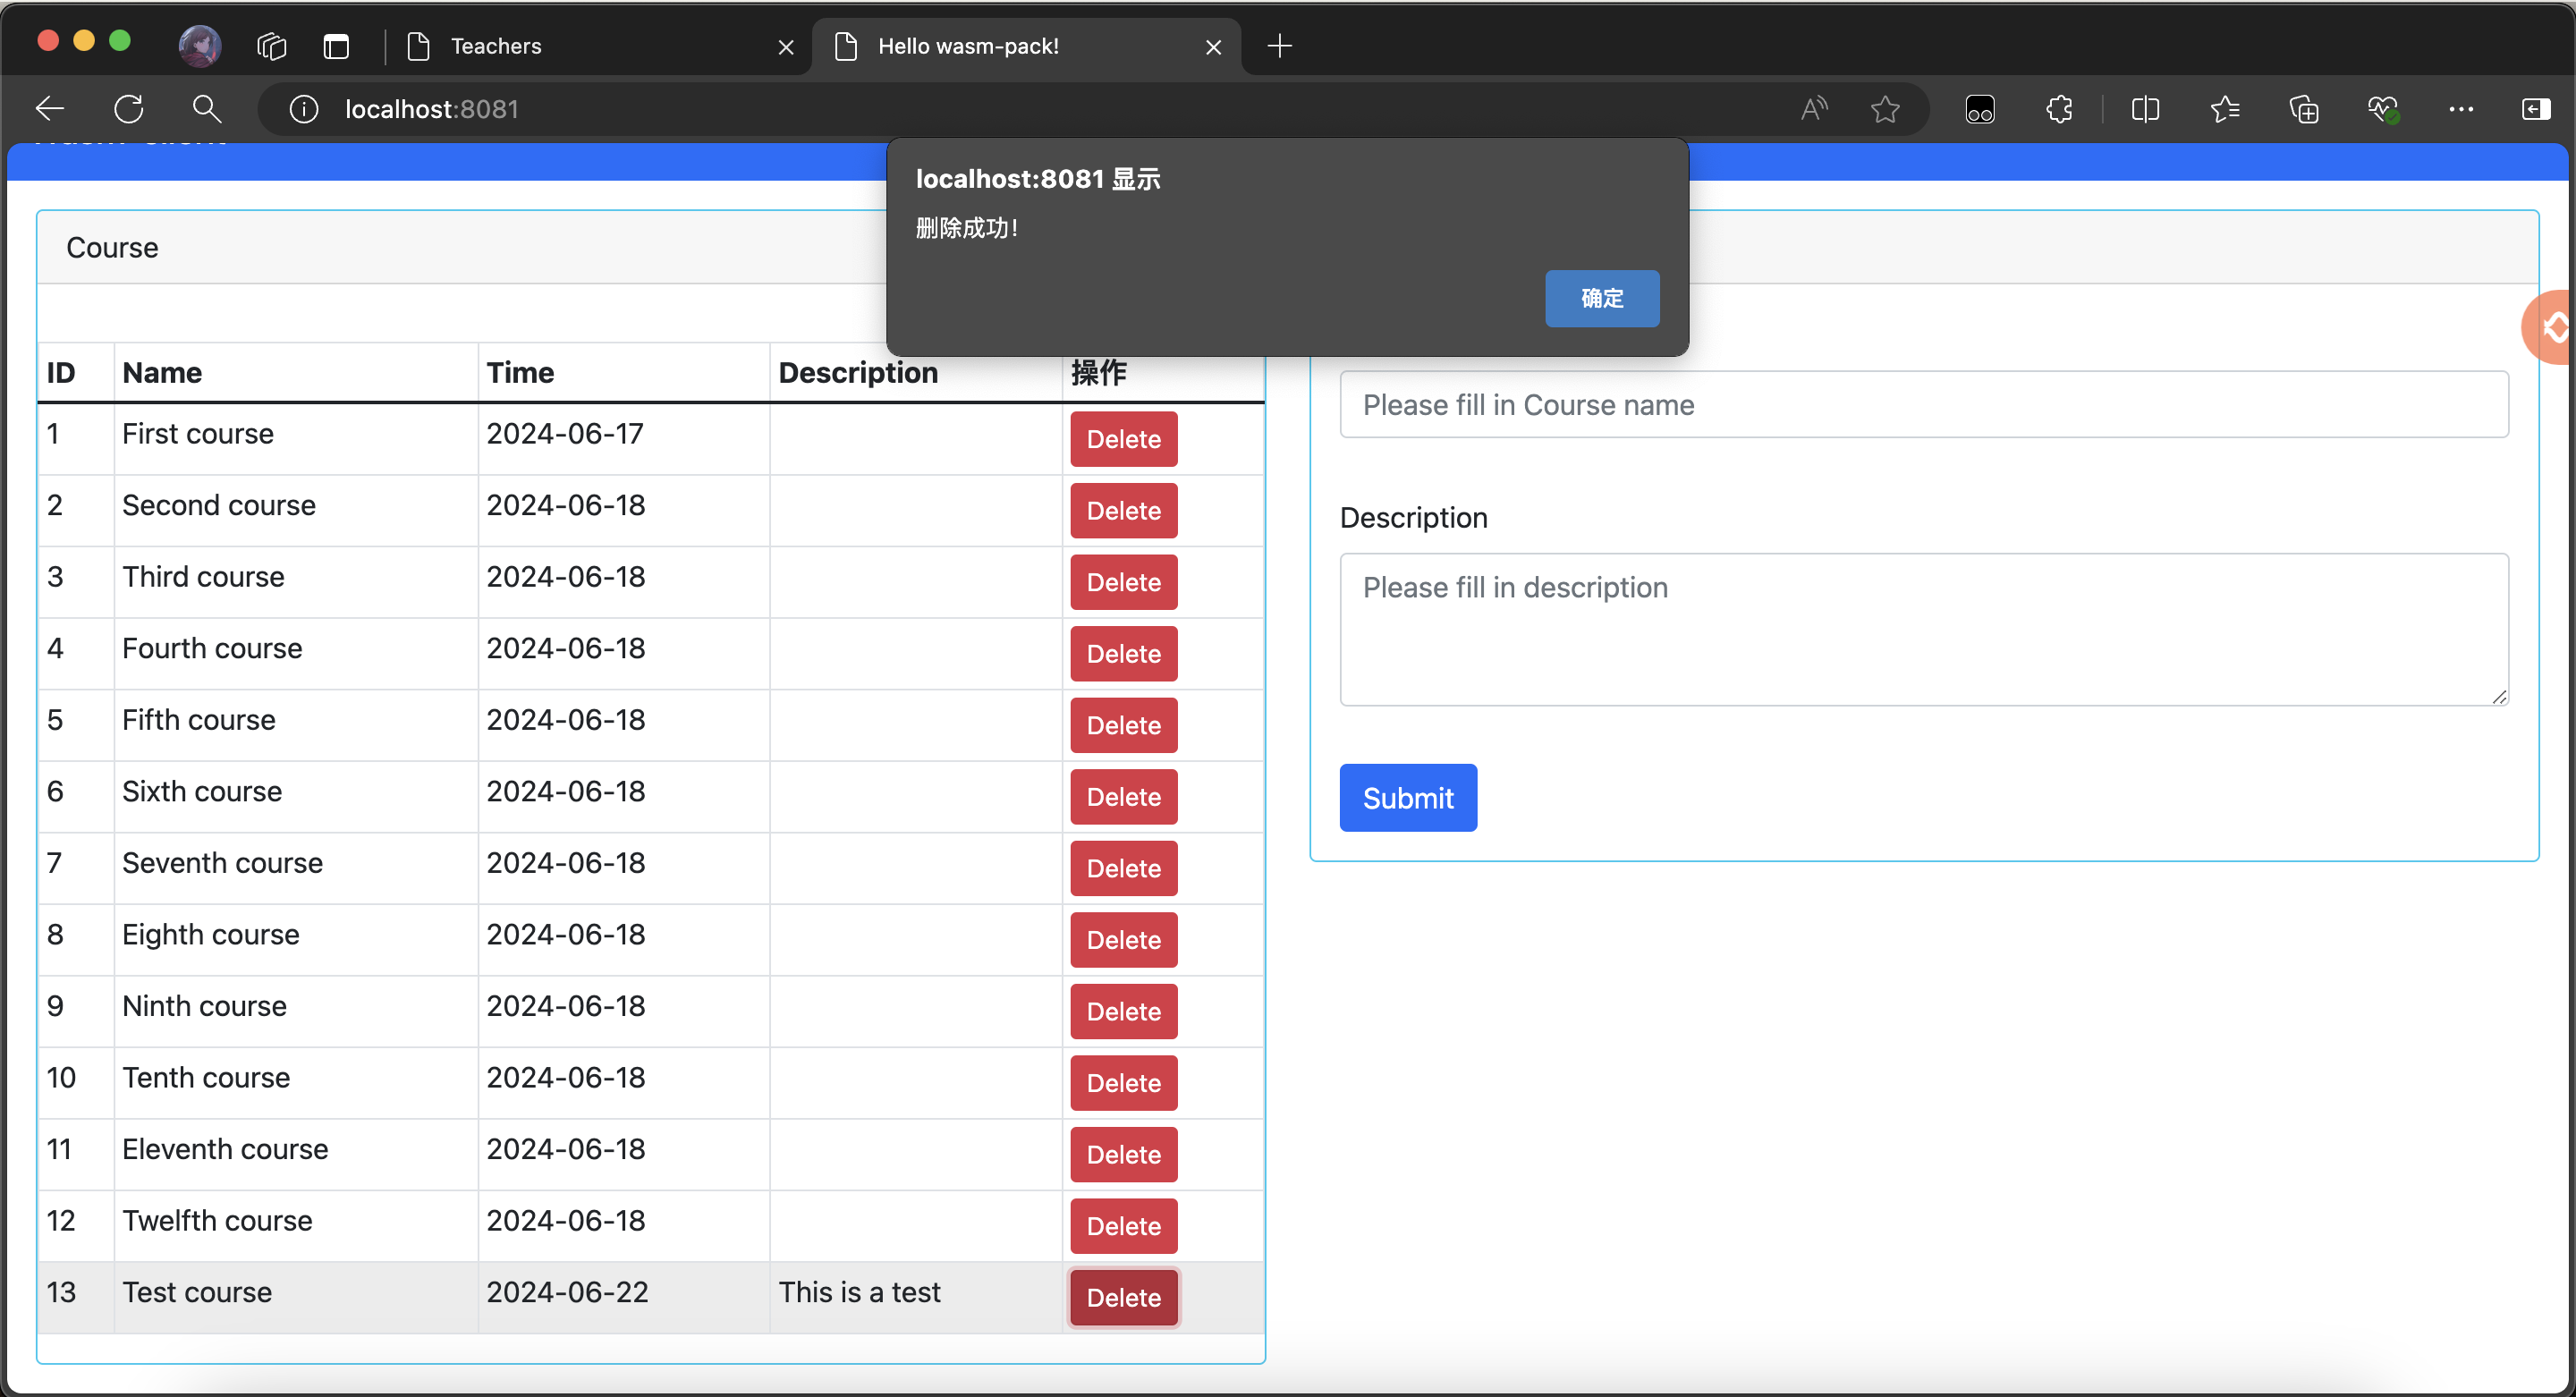
\includegraphics[width=13cm]{images/sec5/Delete_Course_Success.png}
\end{figure}
\newpage
返回课程管理页面,可以看到删除已经成功:
\begin{figure}[!htbp]
    \centering
    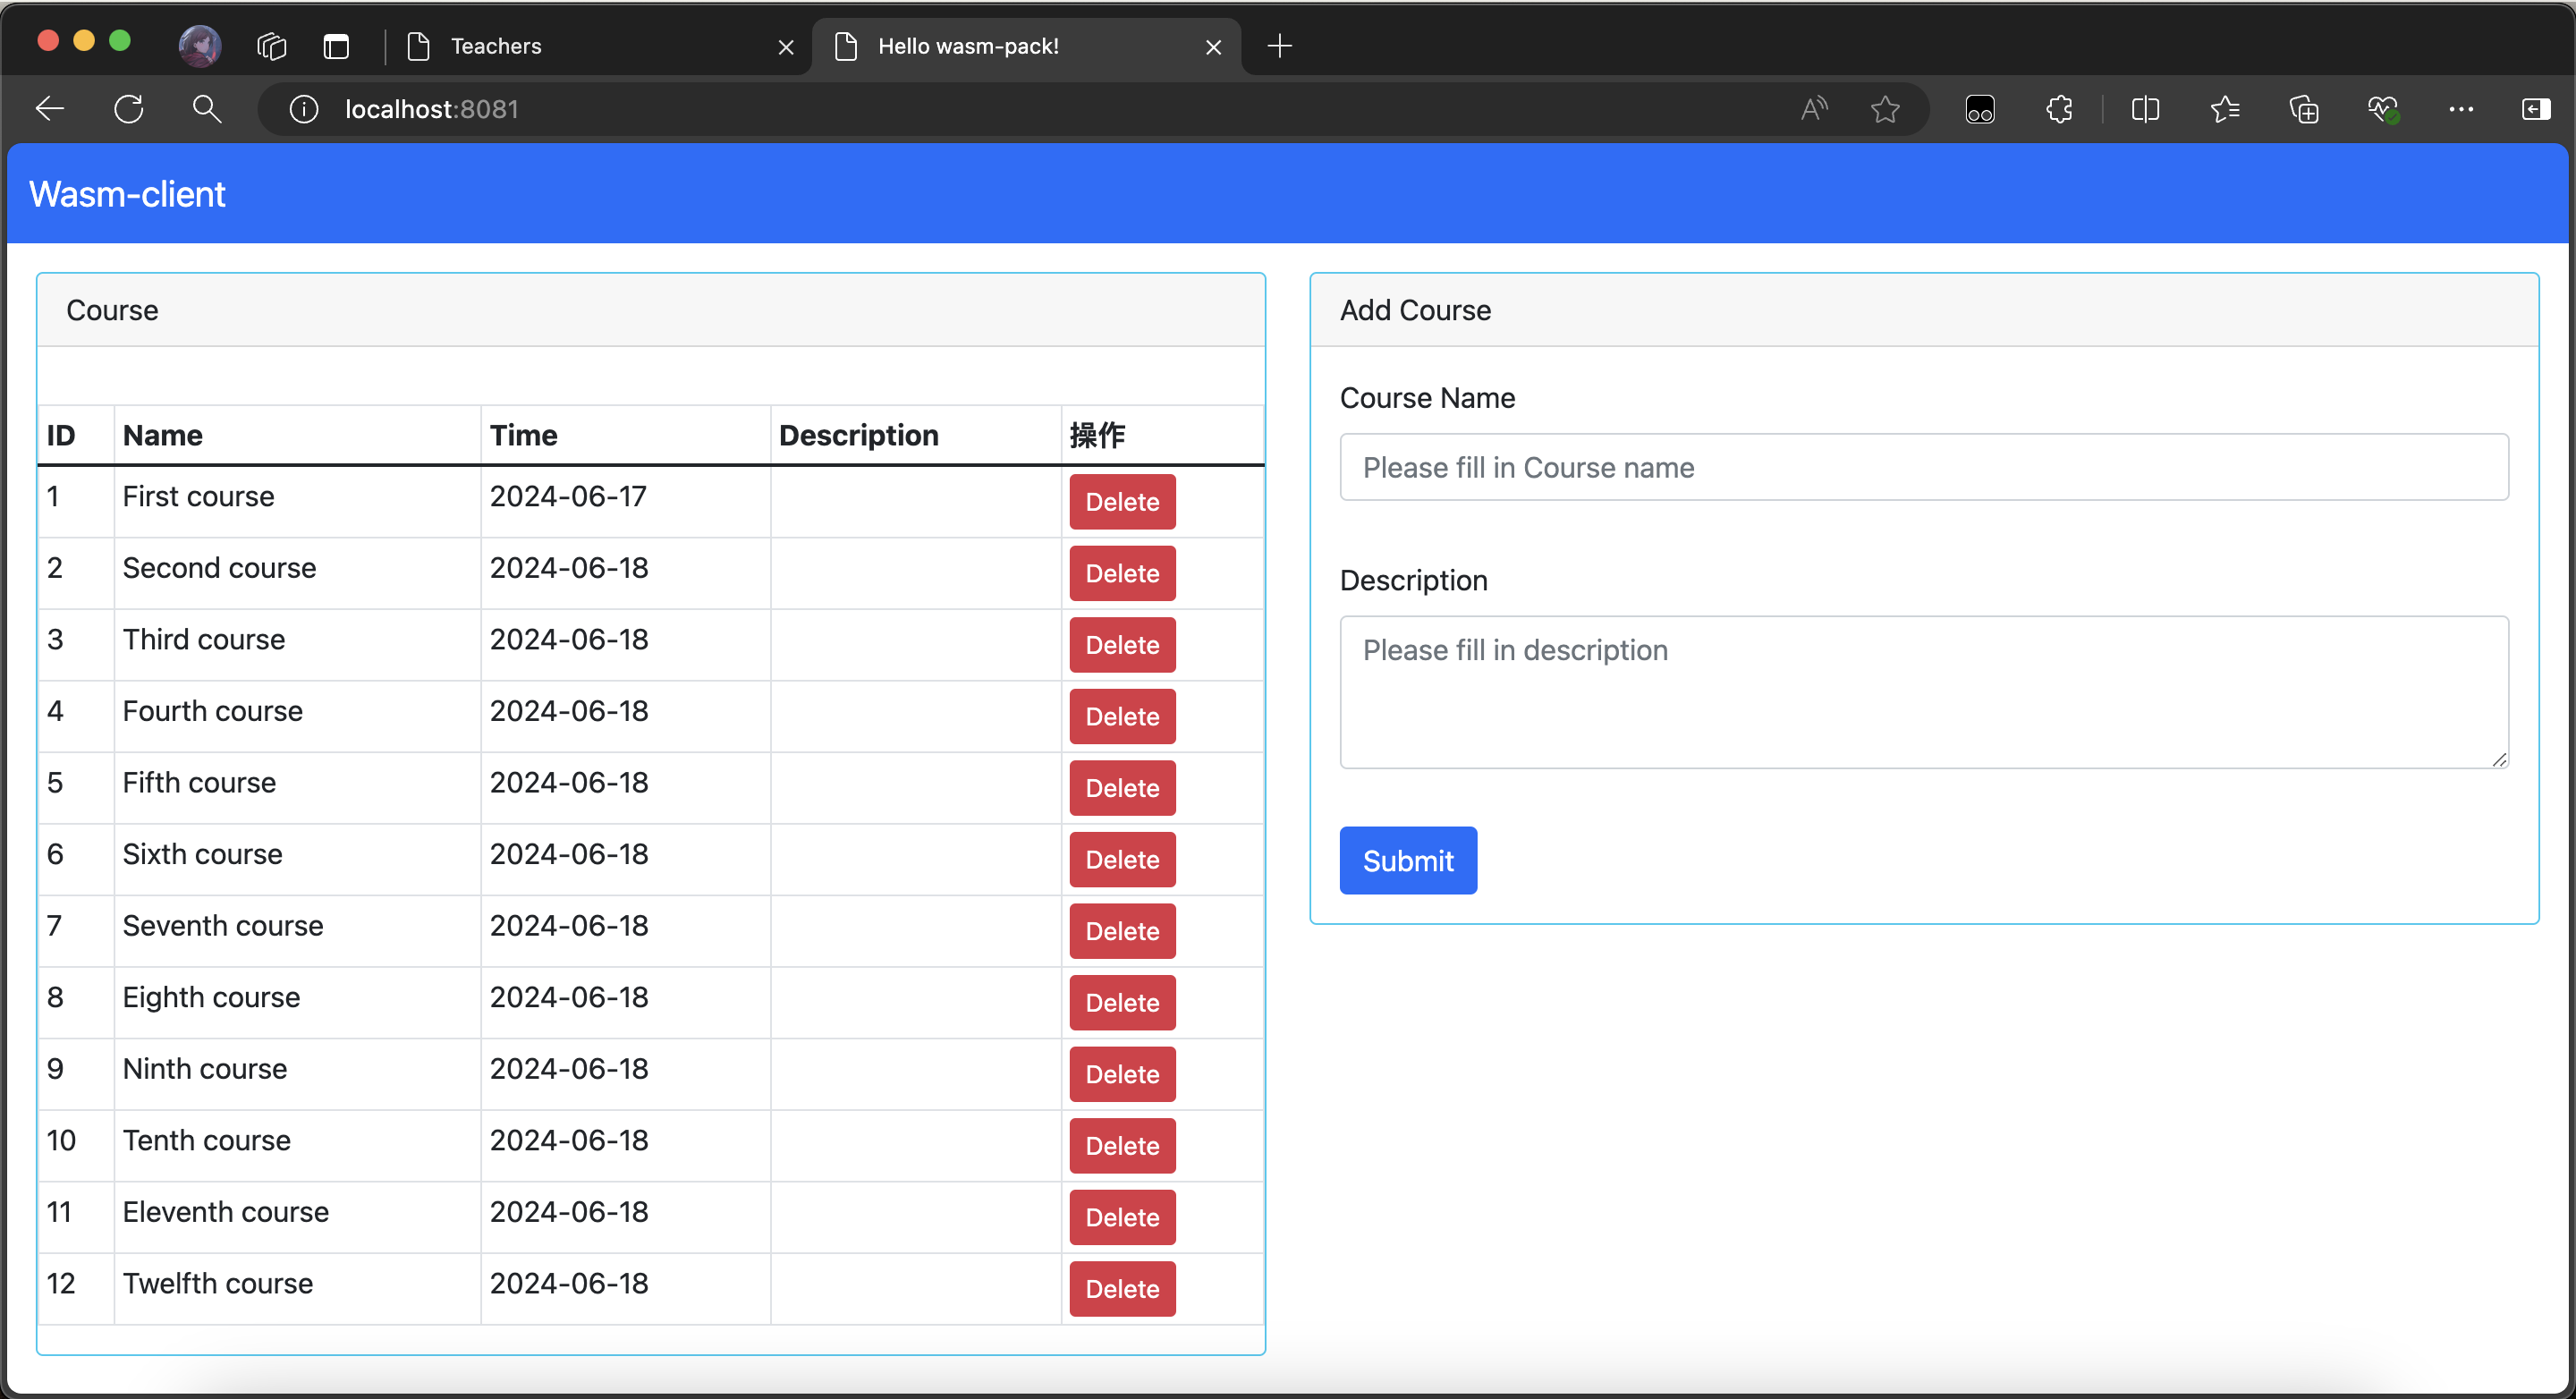
\includegraphics[width=13cm]{images/sec5/Delete_Course_Check.png}
\end{figure}

\subsection{系统设计亮点}

\begin{itemize}
    \item 本项目是一个 Rust 全栈开发项目,使用 Rust 语言编写后端服务,使用 Rust 模板引擎 Tera 渲染教师管理前端页面,同时使用 Web­Assembly 构建课程管理前端页面.
    \item 后端使用 Actix Web 框架,提供了高性能的 Web 服务,同时使用 sqlx crate 访问数据库,实现了课程管理与教师管理两个模块.
    \item 前端使用 Rust 模板引擎 Tera 渲染教师管理页面,使用 Web­Assembly 构建课程管理页面,提供了友好的用户界面.
    \item 整个系统基于阿里云数据库 RDS PostgreSQL Serveless,提供了高可用性、高性能的数据库服务.
\end{itemize}

\newpage

\begin{appendices}
    \renewcommand{\thesection}{\Alph{section}}
    \section{SQL代码}
        \lstinputlisting[
            style       =   SQL,
            caption     =   {\bf 初始化数据库},
            label       =   {init_db}
        ]{./code/init.sql}

        \lstinputlisting[
            style       =   SQL,
            caption     =   {\bf 查询教师表},
            label       =   {teacher_query}
        ]{./code/teacher_query.sql}

        \lstinputlisting[
            style       =   SQL,
            caption     =   {\bf 查询课程表},
            label       =   {course_query}
        ]{./code/course_query.sql}
\end{appendices}

\end{document}